%%%%%%%%%%%%%%%%%%%%%%%%%%%%%%%%%%%%%%%%%
\documentclass[11pt]{report}

% Essential packages
\usepackage[T1]{fontenc}   
\usepackage{lmodern}      
\usepackage{graphicx}
\usepackage{fancyhdr}
\usepackage{fullpage}
\usepackage{amsmath}
\usepackage{caption}
\usepackage{subcaption}
\usepackage{algpseudocode,algorithm}
\usepackage[section]{placeins}
\usepackage{amssymb} 
\usepackage{textcomp}
\usepackage{tocloft}
\usepackage{multicol}
\usepackage{setspace}
\usepackage{enumitem}
\usepackage{hyperref}
\usepackage{tabularx}
\usepackage{listings}
\usepackage{xcolor}
\usepackage{enumitem}
\usepackage{longtable}
\usepackage{float}
\usepackage{tikz}
\usetikzlibrary{arrows.meta, positioning, shapes.geometric, calc, fit}

\onehalfspacing

% Formatting for List of Figures/Tables
\newlength{\mylen}
\renewcommand{\cftfigpresnum}{\figurename\enspace}
\renewcommand{\cftfigaftersnum}{:}
\settowidth{\mylen}{\cftfigpresnum\cftfigaftersnum}
\addtolength{\cftfignumwidth}{\mylen}

\renewcommand{\cfttabpresnum}{\tablename\enspace}
\renewcommand{\cfttabaftersnum}{:}
\settowidth{\mylen}{\cfttabpresnum\cfttabaftersnum}
\addtolength{\cfttabnumwidth}{\mylen}

\begin{document}
\renewcommand\bibname{References}
\pagestyle{fancy}
\fancyhead{}
\fancyfoot{}
\fancyfoot[c]{\thepage}
\fancyfoot[l]{\footnotesize MCA 2024-26}
\renewcommand{\chaptermark}[1]{\markboth{\thechapter.\ #1}{}} 
\renewcommand{\headrulewidth}{0.1pt}
\fancyhead[R]{\footnotesize \nouppercase{\leftmark}}
\fancyhead[L]{\footnotesize IDVision}
\addtolength{\headheight}{\baselineskip}
\addtolength{\headsep}{.1in}

%%%%%%%%%%%%%%%%%%%% TITLE PAGE %%%%%%%%%%%%%%%%%%%%
\begin{titlepage}
\begin{center}

\LARGE{\textbf{Real-Time Detection and Recognition of Missing persons and Criminals}}\\

\vspace{1.0in}
\large{\textbf{Project Report\\}}

\textit{Submitted for the Partial Fulfillment of the Requirements for the Award of the Degree of \textbf{Master of Computer Applications}} \\[2cm]

Submitted by\\[0.5cm]
\textbf{\textsc{ Nussath N }}\\
\textbf{\textsc{Reg No: MUT24MCA-2044}}\\[1cm]

Under the guidance of\\[0.5cm]
\textbf{\textsc{Mr. Sivadas T. Nair}}\\
\textbf{\textsc{Assistant Professor}}\\[1.5cm]


\includegraphics[width=12cm]{mits logo.png}\\[0.5cm]

\textbf{\textsc{DEPARTMENT OF COMPUTER APPLICATIONS}}\\[0.5cm]
\textit{(Affiliated to APJ Abdul Kalam Technological University)}\\
{\upshape \textbf{MARCH 2026}} % mention the month of your presentation.
\end{center}
\end{titlepage}

%%%%%%%%%%%%%%%%%%%% CERTIFICATE %%%%%%%%%%%%%%%%%%%%
\begin{titlepage}
\begin{center}

\includegraphics[width=10cm]{mits logo.png}\\[0.5cm]
{\large \textbf{ Varikoli P.O., Puthencruz-682308}}\\[1cm]
\textbf{\textsc{DEPARTMENT OF COMPUTER APPLICATIONS}}\\[2cm]
\textsc{\textbf{\LARGE BONAFIDE CERTIFICATE}}\\[2cm]
\end{center}
This is to certify that the project report entitled " Real-Time Detection and Recognition of Missing persons and Criminals" has been submitted by \textbf{Nussath N (Reg no : MUT24MCA-2044)} is a bonafide account of the work done by her under our supervision for the partial fulfillment of the requirements for the award of the degree of Master of Computer Applications (MCA) of A P J Abdul Kalam Technological University, Kerala during the academic year 2025-26.\\[2cm]

\flushleft{\textbf{Guide}}\hspace{4cm}\textbf{Coordinator(s)}\hspace{3.5cm}\textbf{Head of the Department}\\
Mr. Sivadas T Nair\hspace{1.9cm}Mr. Sivadas T Nair, Dr Geethu S\hspace{2cm}Dr Saritha K\\
Asst. Professor\hspace{2.5cm}Asst. Professors\hspace{4.9cm} Professor\\
Dept. of CA\hspace{3.1cm}Dept. of CA\hspace{5.5cm} Dept. of CA\\[1cm]
Submitted for the Final Evaluation held on ………………\\[1.5cm]
\hspace{8cm} Name and Signature of the Examiner
\end{titlepage}

%%%%%%%%%%%%%%%%%%%% ACKNOWLEDGEMENT %%%%%%%%%%%%%%%%%%%%
\begin{titlepage}
\begin{center}
\Large{\textbf{Acknowledgements}}\\[1cm]
\end{center}
\normalsize 
This project is the result of my hard work wherein I have been helped and supported by several persons and institutions directly and indirectly. Now it is the time to acknowledge their contributions.\par
Foremost, I would like to express my sincere gratitude to my project guide, \textbf{Asst./Prof. Sivadas T Nair} for his continuous encouragement, invaluable guidance, motivation and enthusiasm throughout my project. \par
My sincere gratitude to \textbf{Dr. Saritha K}, Head of Department during my course period 2024-2026. I would also like to thank the project coordinator(s) \textbf{Sivadas T Nair} and \textbf{Dr. Geethu S} for critically assessing my work and giving valuable suggestions. I would like to acknowledge management of Muthoot Institute of Technology \& Science for providing academic support to complete my project.\par
In my daily work I have been blessed with a friendly and cheerful group of fellow students. I am very much thankful to all the members of S4 MCA.\par
Besides this, several people have knowingly and unknowingly helped me in the successful completion of this project. I express my sincere gratitude to all of them.

\begin{flushright}
Nussath N
\end{flushright}
\end{titlepage}

%%%%%%%%%%%%%%%%%%%% ABSTRACT %%%%%%%%%%%%%%%%%%%%%%%
\begin{titlepage}
\begin{center}
\textsc{\textbf{\LARGE Abstract}}\\[2cm]
\end{center}
\pagenumbering{roman}
The process of manual surveillance traditionally relies on continuous human monitoring, which can be inefficient, error-prone, and difficult to scale in real-world environments. To address these limitations, this project introduces IDVision, a comprehensive AI-powered surveillance system designed to provide automated, real-time identification of individuals from live video streams and recorded footage. By leveraging advanced computer vision and deep learning techniques, the system delivers accurate and data-driven detection of missing persons and criminal suspects.


The core analytical engine integrates multiple stages of visual processing to ensure reliable performance. In the live web pipeline, face detection is performed by the YuNet face detector (an ONNX model loaded through OpenCV's \texttt{FaceDetectorYN}), which is robust to pose and lighting variations. Each detected face is cropped, converted to grayscale, resized to 200$\times$200, and passed to a Local Binary Patterns Histograms (LBPH) recogniser trained on a custom dataset of missing persons and criminal suspects. A per-label streak filter suppresses flickery false positives by requiring the same label to be predicted in at least three of the last five frames before accepting a match, and a per-(name, category) cooldown prevents redundant alerts. A lightweight blur-variance heuristic provides a basic liveness check in the standalone recogniser, while a CNN-based liveness model is flagged as a future upgrade.


The architectural framework consists of a high-performance FastAPI backend integrated with a SQLite database for secure and persistent data management. Authentication is handled by bcrypt-hashed passwords and signed session cookies, and all mutating routes enforce role-based access control (admin vs.\ viewer). The client side is a Jinja2-rendered dashboard that enables authorised users to monitor the live feed, enrol new individuals with validated photo uploads, retrain the recognition model from the browser, and review detection logs. On a positive match the system writes a structured row to the alerts table, appends to a plain-text log, and dispatches an email through SMTP on a background thread so slow mail servers never stall the camera loop.


The dataset used in this project is a custom-built collection of labeled facial images organized by individual and category, enabling supervised learning. The performance of the system is evaluated using standard metrics such as accuracy, confusion matrix, and classification report, providing insights into recognition effectiveness. By integrating deep learning-based face recognition with a scalable web framework, IDVision bridges the gap between advanced machine learning techniques and practical surveillance applications, delivering an efficient and automated solution for modern security systems.
\end{titlepage}

%%%%%%%%%%%%%%%%%%%% TOC, LISTS %%%%%%%%%%%%%%%%%%%%
\tableofcontents
\cleardoublepage
\addcontentsline{toc}{chapter}{\listfigurename}
\listoffigures
\cleardoublepage
\addcontentsline{toc}{chapter}{\listtablename}
\listoftables
\cleardoublepage

\section*{List of Abbreviations}

\begin{tabular}{ll}
CV & Computer Vision \\
DNN & Deep Neural Network \\
API & Application Programming Interface \\
LBPH & Local Binary Patterns Histograms \\
LBP & Local Binary Pattern \\
ONNX & Open Neural Network Exchange \\
SMTP & Simple Mail Transfer Protocol \\
RBAC & Role-Based Access Control \\
ORM & Object--Relational Mapping \\
\end{tabular}

\newpage

%%%%%%%%%%%%%%%%%%%% MAIN CHAPTERS %%%%%%%%%%%%%%%%%%%%
\pagenumbering{arabic}

\chapter{Introduction}
\section{Definition \& Problem Statement}
IDVision is a full-stack, AI-powered surveillance system designed to automatically detect and recognise individuals from live video streams. It uses OpenCV's YuNet deep face detector to locate faces in live webcam frames and a Local Binary Patterns Histograms (LBPH) recogniser trained on a custom dataset to identify known missing persons and criminal suspects. A per-label temporal streak filter, a confidence threshold, and a per-person cooldown together keep false-positive alerts under control, and a lightweight blur-variance check is retained as a placeholder liveness gate for a planned CNN-based liveness upgrade.

In traditional surveillance systems, the most significant challenge lies in the reliance on continuous human monitoring, which is both inefficient and prone to error. Security personnel are required to observe multiple video feeds simultaneously, making it difficult to consistently detect suspicious individuals or identify missing persons in real time. This often leads to delayed responses, overlooked threats, and increased operational burden. Furthermore, manual identification depends heavily on human memory and attention, which can vary under fatigue or high workload conditions.

Existing surveillance solutions may provide basic video recording or motion detection but lack intelligent, automated identification capabilities. There is a clear need for a system that can not only detect faces but also verify their authenticity and accurately recognize individuals with minimal human intervention. Such a system should be capable of generating real-time alerts, providing actionable insights, and maintaining a structured record of detected events. By addressing these limitations, IDVision aims to deliver a scalable and efficient solution for modern surveillance challenges, enhancing both accuracy and response time in security-critical environments.
\section{Background and Motivation}

With the rapid growth of urbanization and increasing security concerns, the need for efficient surveillance systems has become more critical than ever. Traditional monitoring methods rely heavily on human observation through CCTV footage, which is time-consuming, error-prone, and often ineffective in real-time threat detection. Identifying missing persons or criminal individuals manually from continuous video streams is a challenging task and can lead to delayed responses.

Moreover, conventional systems lack the capability to verify whether a detected face is real or a spoof attempt using photos or videos, raising serious security vulnerabilities. This creates a strong need for an intelligent system that can automatically detect, verify, and recognize individuals in real-time with high accuracy.

The motivation behind IDVision is to develop an AI-powered surveillance system that integrates face detection, liveness detection, and face recognition into a unified framework. By leveraging advanced computer vision and deep learning techniques, the system aims to provide fast, reliable, and automated identification of individuals, thereby enhancing security, reducing human effort, and enabling timely decision-making in critical situations.


\subsection{Scrum}

Scrum is an agile framework for managing complex projects, mostly applied in software development but may be applied in other fields. It focuses on iterative progress, flexibility, and cohesiveness among team members, enabling teams to provide high-value products incrementally and requiring frequent feedback and adjustments.

\subsubsection*{Key Components of Scrum:}

\paragraph{Roles:}
\begin{itemize}
    \item \textbf{Product Owner:} Defines product features/functionalities, prioritizes tasks, and keeps them aligned with business goals.
    \item \textbf{Scrum Master:} Facilitates the Scrum process, removes impediments, and ensures practices of Scrum.
    \item \textbf{Development Team:} Interdisciplinary team who actually do the work to produce potentially shippable product increments at the end of each sprint.
\end{itemize}

\paragraph{Artifacts:}
\begin{itemize}
    \item \textbf{Product Backlog:} The Prioritised list of tasks, features or user stories defining the work in the project.
    \item \textbf{Sprint Backlog:} Selection from the product backlog for a sprint; Expected to be completed during the sprint.
    \item \textbf{Increment:} The total of all product backlog items that were accomplished within a sprint and all sprints leading up to it.
\end{itemize}

\paragraph{Events:}
\begin{itemize}
    \item \textbf{Sprint:} A time-boxed sequence, typically from 1 to 4 weeks, during which the development team will work on achieving a quantity of work from the sprint backlog.
    \item \textbf{Sprint Planning:} A meeting at the beginning of a sprint that involves the team's decisions as to which tasks in the product backlog they will execute during the sprint.
    \item \textbf{Daily Scrum (Stand-up):} A short usually 15 minutes meeting where members report on work done, work planned, and difficulties encountered.
    \item \textbf{Sprint Review:} A meeting held by the end of each sprint to be able to show what has been achieved and obtain feedback.
    \item \textbf{Sprint Retrospective:} A reflective meeting where the team discusses successes, challenges, and areas for improvement for the next sprint.
\end{itemize}

\paragraph{Scrum Values:}
\begin{itemize}
    \item Commitment
    \item Focus
    \item Openness
    \item Respect
    \item Courage
\end{itemize}

\noindent Scrum encourages continuous improvement and change, plus teamwork, therefore this is one of the reasons why many teams benefit from working in dynamic and constantly changing environments.
\begin{figure}[!ht] 
    \centering
    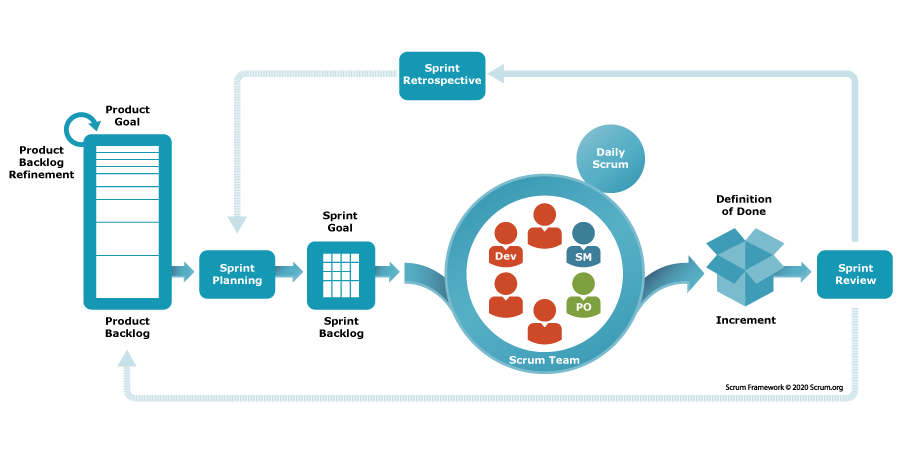
\includegraphics[height=10cm, width=17cm]{scrum-framework.png}
    \caption{Scrum}
    \label{Fig1}
\end{figure}
\subsection{ Implementation of Scrum in the Project }

\begin{figure}[H]
	\centering
	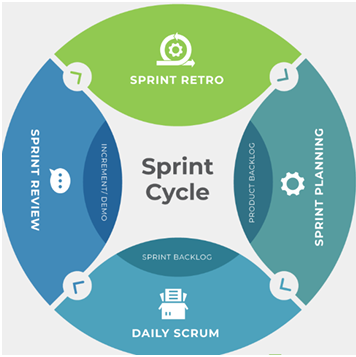
\includegraphics[width=6cm, height=6cm]{SprintCycle.png}
	\caption{ Agile Sprint Cycle }
	\label{fig: Agile Sprint Cycle }
\end{figure}

In this project, the Scrum framework was tailored to support effective progress tracking, rapid prototyping, and regular feedback incorporation. Here’s how it was implemented across the development cycle:

\begin{enumerate}
    \item \textbf{Sprint Planning:}  At the beginning of each sprint, the team held a sprint planning session to review the project backlog, prioritize tasks, and set sprint goals. Tasks were broken down into manageable items, assigned story points based on complexity, and selected for the sprint backlog. This ensured that each sprint had a clear objective and that the workload was feasible within the sprint’s timeframe. 
    \item \textbf{Daily Stand-up Meetings:} Daily stand-ups were held every morning to discuss progress, blockers, and upcoming tasks. These brief meetings, typically lasting 15 minutes, allowed team members to stay aligned and quickly address any issues impeding progress. By maintaining open communication and transparency, the team minimized misunderstandings and fostered a collaborative environment. 
    \item \textbf{Backlog Refinement Sessions:} The product backlog was revisited regularly in backlog refinement sessions. This process involved evaluating new requirements, reprioritizing tasks, and adding details to user stories to clarify objectives. By refining the backlog consistently, the team could respond to new insights, adjust the project roadmap, and ensure that high-priority tasks were always well-defined for upcoming sprints. 
    \item \textbf{Sprint Review:}At the end of each sprint, a sprint review was conducted to demonstrate the work completed. This allowed stakeholders to view the latest product increment and provide feedback on features or adjustments needed. The review ensured that any necessary changes were identified and scheduled for the next sprint, supporting continuous improvement and alignment with stakeholder expectations. 
     \item \textbf{Sprint Retrospective:}After the sprint review, a sprint retrospective was held to reflect on the sprint process itself. This ceremony provided a platform for the team to discuss what went well, what could be improved, and how to apply lessons learned in the following sprint. By embracing a culture of continuous improvement, the team could fine-tune its processes to boost efficiency and quality in each successive sprint.
      \item \textbf{Continuous Feedback Loop:}Feedback was collected and incorporated throughout the project, enabling rapid prototyping and allowing the team to make adjustments based on testing outcomes. This approach not only enhanced the end product's quality but also ensured that the final system aligned closely with user needs and expectations.  
\end{enumerate}

\subsection{Burndown Chart}
A burndown chart is an essential visual tool in Agile and Scrum project management, used to track the progress of work over a sprint. It represents the remaining work (or "burndown") over time, providing a straightforward way to gauge whether the team is on track to complete the planned tasks by the end of the sprint. Burndown charts are particularly valuable for both
team members and stakeholders as they offer real-time insights into the pace of work and help identify potential bottlenecks early.

The burndown chart is typically a line graph with two main axes: 
\begin{itemize}
    \item X-Axis: Represents the time period of the sprint (usually in days).  
    \item Y-Axis: Represents the amount of remaining work, usually measured in story points, tasks, or hours.
\end{itemize}

The chart starts with the total work at the beginning of the sprint and ideally trends downward to zero as tasks are completed. This downward trajectory shows the team’s progress over time. 

\begin{figure}[H]
	\centering
	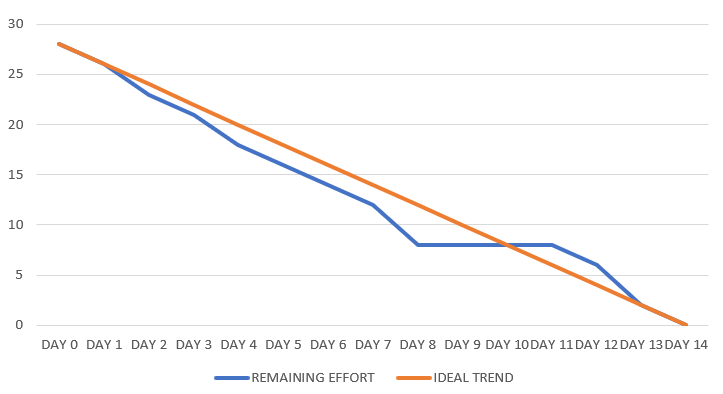
\includegraphics[width=12cm, height=8cm]{SampleBurndownChart.png}
	\caption{  Sample Burndown Chart }
	\label{fig:Sample Burndown Chart  }
\end{figure}

In a standard burndown chart:
\begin{itemize}
    \item The ideal burndown line represents the steady progress needed to complete all tasks by the end of the sprint. This line assumes that tasks are completed at a constant pace throughout the sprint. 
    \item The actual burndown line tracks the real progress of the team, showing the actual amount of remaining work each day. When the actual line diverges from the ideal line, it can indicate issues or delays that need attention. 
\end{itemize}

In this project, a burndown chart was used throughout each sprint to provide a clear picture of the team’s progress and to monitor whether the sprint goals were achievable. Here’s how it helped at each stage.
\begin{itemize}
    \item Tracking Daily Progress: During the sprint, the team updated the chart daily, logging the completed tasks and adjusting the remaining workload. This practice enabled the team to visualize whether they were  keeping up with the expected pace and whether any adjustments were needed  
    \item Identifying Bottlenecks: If the actual burndown line began to lag significantly behind the ideal line, it indicated potential bottlenecks or issues within the sprint. This visibility allowed the team to address these issues promptly, such as reallocating resources or revising the sprint scope if necessary 
   \item Promoting Transparency and Accountability: The burndown chart provided a transparent view of progress for all stakeholders. By sharing the chart in daily standups and sprint reviews, team members could discuss any gaps between planned and actual progress and collectively strategize to overcome any obstacles. This transparency fostered accountability and empowered the team to take proactive measures 
   \item Facilitating Retrospective Analysis: At the end of each sprint, the burndown chart was reviewed during the sprint retrospective. By analysing patterns, the team could assess what went well and identify areas for improvement. For example, if the team consistently struggled to meet the ideal burndown rate in the latter half of sprints, they might consider adjusting task estimates or prioritization strategies 
\end{itemize}

\section{Significance}
The primary significance of IDVision lies in the automation and enhancement of traditional surveillance systems through intelligent, data-driven decision-making. By eliminating the need for continuous manual monitoring, the system enables real-time detection and identification of individuals with improved accuracy and consistency, thereby reducing human error and operational burden. The integration of liveness detection further strengthens system reliability by preventing spoofing attempts such as photographs or video replays. By transforming complex visual data into actionable alerts and structured logs, 
IDVision allows security personnel to respond quickly to critical situations, including the identification of missing persons and criminal suspects. Additionally, the centralized dashboard facilitates efficient monitoring and analysis, while the scalable and cost-effective architecture makes the system suitable for deployment in various real-world environments such as public spaces, transportation hubs, and institutional settings. Overall, IDVision bridges the gap between advanced computer vision technologies and practical surveillance needs, contributing to improved safety, efficiency, and decision-making in modern security systems.

\section{Uses and Scope}
\textbf{Uses:}
\begin{itemize}
    \item \textbf{Law Enforcement Agencies:} Police departments can utilize the system to identify missing persons and criminal suspects in real time, improving response time and investigation efficiency.
    \item \textbf{Public Surveillance Systems:} The system can be deployed in locations such as airports, railway stations, and public spaces to enhance security through automated monitoring and alert generation.
    \item \textbf{Institutional Security:} Organizations such as universities, offices, and residential complexes can use the system for controlled access and monitoring unauthorized individuals.
\end{itemize}
\textbf{Scope:} \\
The current scope of IDVision focuses on real-time and offline video-based face detection, liveness verification, and identity recognition using a custom dataset. It processes input from live cameras or uploaded videos, generates alerts for predefined categories, stores event logs, and provides a web-based dashboard for monitoring. Advanced features such as multi-camera tracking and large-scale deployment are beyond the scope of this implementation.

\section{Contribution}
This project contributes a practical integration of computer vision, deep learning, and full-stack web technologies within an intelligent surveillance framework. Specifically, the contributions include:
\begin{enumerate}
    \item \textbf{Real-Time Recognition Pipeline:} Implementing a face recognition pipeline that couples the YuNet deep face detector (via OpenCV's \texttt{FaceDetectorYN}) with an LBPH recogniser trained on a custom dataset, along with a per-label streak filter and confidence threshold that together suppress the flickery false positives characteristic of small-dataset LBPH models.
    \item \textbf{Secure, Role-Based Web Application:} Building a FastAPI application with bcrypt-hashed credentials, signed session cookies, role-based access control (admin vs.\ viewer), bootstrap-gated registration, and magic-byte validation of photo uploads, deployed behind a Jinja2 dashboard that an admin can use to enrol new individuals and retrain the recogniser in-process.
    \item \textbf{Intelligent Alert Mechanism:} Developing a category-aware alert subsystem that writes every match to the SQLite alerts table, appends to a plain-text log, and dispatches email notifications over SMTP in a background thread, all gated by a per-(name, category) cooldown so a single prolonged detection does not flood the inbox or the log.
\end{enumerate}

\section{Objectives}
The core objectives of the IDVision project are:
\begin{itemize}
    \item To design and implement a robust face detection system using computer vision techniques for accurate identification of faces in images and video streams.
    \item To develop a reliable liveness detection module to distinguish between real faces and spoofing attempts such as photos or videos.
    \item To create an interactive web-based dashboard that enables real-time monitoring, alert visualization, and management of surveillance data.
    \item To design a scalable system architecture that can be extended for future enhancements such as multi-camera tracking and cloud deployment.
    \item To generate automated alerts for identified missing persons and criminal suspects, improving response time in critical situations.
\end{itemize}

\section{Organization of the Report}
The remainder of this report is organized as follows:
\begin{itemize}
    \item \textbf{Chapter 2: Literature Review} explores existing research in face detection, liveness detection, and deep learning-based face recognition techniques relevant to surveillance systems.
    \item \textbf{Chapter 3: System Analysis and Design} details the overall architecture, system workflow, database design, and the core logic behind detection, recognition, and alert generation.
    \item \textbf{Chapter 4: Implementation} discusses the technologies, frameworks, and libraries used to develop the FastAPI backend, computer vision modules, and the web-based dashboard.
    \item \textbf{Chapter 5: System Testing} outlines the testing methodologies used to evaluate the accuracy of face recognition, performance of the liveness detection module, and reliability of the alert system..
    \item \textbf{Chapter 6: Conclusion and Future Enhancements} summarizes the project’s achievements and discusses potential future upgrades to the IDVision  ecosystem.
\end{itemize}


\chapter{LITERATURE REVIEW}  
This chapter explores the foundational concepts, existing methodologies, and technological advancements that form the basis of the IDVision system. The literature reviewed encompasses face detection techniques, liveness detection mechanisms, and deep learning-based face recognition models used in modern surveillance systems. By analyzing previous research, this section identifies the limitations of traditional monitoring approaches and establishes the theoretical framework for the proposed intelligent surveillance solution.
\section{Related Works}
The paper “Face Recognition Using Deep Learning: A Survey” provides a comprehensive overview of modern face recognition techniques based on deep neural networks. The study highlights the transition from traditional methods such as Eigenfaces and LBPH to deep learning-based embedding models, which offer significantly higher accuracy and robustness. It emphasises the use of feature vectors to represent facial characteristics and compares similarity using distance metrics. This research is relevant to IDVision in two ways: it grounds the current LBPH baseline in the lineage of classical recognition techniques, and it motivates the future-work path of replacing LBPH with a deep-embedding recogniser (such as FaceNet, ArcFace, or dlib's 128-dimensional embedding) for improved robustness to lighting, pose, and facial expression. [3]

Another relevant study, “Real-Time Face Recognition System Using Deep Learning”, explores the implementation of real-time recognition systems using convolutional neural networks. The paper discusses challenges such as latency, computational efficiency, and real-world deployment constraints. It demonstrates how optimized models can achieve a balance between speed and accuracy for live video processing. This work directly supports the design of IDVision, particularly in achieving efficient real-time performance while maintaining reliable identification in both live camera feeds and recorded video analysis. [4]

The paper “Face Liveness Detection with Feature Discrimination Between Sharpness and Blurriness” by C-H. Yeh and H-H. Chang (2017) proposes a novel approach for detecting spoofing attacks by analyzing depth-of-field (DOF) variations in facial images. The study leverages the natural difference in sharpness between facial regions, such as the nose and cheeks, to distinguish real faces from printed photographs. By extracting blur and gradient-based features and applying a K-Nearest Neighbors (KNN) classifier, the system achieves an accuracy of 94.67% in detecting photo-based spoofing attempts. This work is particularly relevant to IDVision, as it highlights alternative lightweight liveness detection strategies based on image quality analysis, complementing deep learning-based approaches and reinforcing the importance of incorporating robust anti-spoofing mechanisms in real-time surveillance systems. [7]

The paper “A Study on Face Recognition Under Varying Illumination Conditions” investigates the impact of lighting variations on recognition accuracy. The study highlights that traditional methods struggle under inconsistent lighting, whereas deep learning-based approaches show improved adaptability. Techniques such as histogram equalisation and feature normalisation are discussed to enhance robustness. These findings are relevant to IDVision because the $200\times200$ grayscale crops fed to LBPH already apply uniform preprocessing, and because the findings further reinforce the case for migrating to deep-embedding recognition as surveillance conditions grow more varied. [5]

In addition, the study “Smart Surveillance Systems Using Artificial Intelligence” examines the integration of computer vision and AI for automated monitoring in public spaces. The paper discusses the role of intelligent alert systems, real-time detection, and centralized dashboards in improving surveillance efficiency. It also highlights the importance of reducing human dependency in monitoring tasks. This research aligns closely with IDVision, as it validates the system’s architecture, which combines automated detection, recognition, and alert generation with a web-based dashboard for efficient monitoring and management. [6]



\chapter{TECHNICAL STACK} 
\section*{Existing System}

Traditional surveillance systems primarily rely on continuous monitoring through CCTV cameras, where human operators manually observe video feeds to identify suspicious activities or individuals. This process is time-consuming, labor-intensive, and highly prone to human error, especially when monitoring multiple video streams simultaneously.

In many cases, existing systems lack intelligent automation and depend on manual identification, making it difficult to detect missing persons or criminal individuals in real time. Additionally, these systems are unable to verify whether a detected face is genuine or a spoof attempt using photographs or videos, which creates serious security vulnerabilities.

Furthermore, conventional approaches do not provide real-time alert mechanisms or efficient data management. Important events may go unnoticed due to delayed human response, and there is often no structured way to store and retrieve detection history. These limitations highlight the need for an automated, intelligent surveillance system capable of accurate detection, recognition, and alert generation.

\section*{3.2 Proposed Methodology}

The \textit{IDVision} system proposes an AI-based approach to overcome the limitations of traditional surveillance systems. The system integrates face detection, liveness detection, and face recognition techniques into a unified pipeline to ensure accurate and secure identification.

The workflow of the proposed system is as follows:

\begin{enumerate}
    \item \textbf{Data Collection:} A dataset of missing persons and criminal suspects is collected and organised into a two-level folder structure (\texttt{dataset/criminals/\{id\}\_\{Name\}/} and \texttt{dataset/missing\_persons/\{id\}\_\{Name\}/}), where each person has multiple face images captured under different conditions.

    \item \textbf{Data Preprocessing (training):} Each dataset image is loaded with OpenCV, the Haar Cascade \texttt{haarcascade\_frontalface\_default.xml} is used to locate the face region, the crop is converted to grayscale and resized to 200$\times$200, and the resulting samples are fed to the LBPH trainer.

    \item \textbf{Face Detection (live feed):} Faces are detected in the webcam stream using OpenCV's YuNet detector (\texttt{FaceDetectorYN}) loaded from the ONNX model \texttt{face\_detection\_yunet\_2023mar.onnx}. YuNet is used here rather than Haar because it is more robust to pose, lighting, and occlusion in live video.

    \item \textbf{Liveness Heuristic:} A lightweight blur-variance check (variance of the Laplacian) is retained in the standalone recogniser as a basic spoofing defence. A proper CNN-based liveness model is listed as a planned upgrade.

    \item \textbf{Face Recognition:} Each detected face region is cropped, grayscaled, resized to 200$\times$200, and passed to the LBPH recogniser. The predicted label is resolved to a (name, category) pair via an enriched label map that embeds the category for each label, which avoids the id-collision problem caused by the criminals and missing-persons tables having independent auto-increment counters.

    \item \textbf{Streak Filter and Thresholding:} The raw prediction is only accepted as a match if its LBPH confidence is below a configurable threshold \emph{and} the label has appeared in at least $K$ out of the last $N$ predictions (defaults $K=3$, $N=5$). This suppresses the flickery false positives LBPH tends to produce on small datasets.

    \item \textbf{Alert Generation and Storage:} When a match passes the threshold and streak checks, the system writes a row to the SQLite \texttt{alerts} table, appends a line to \texttt{alerts\_log.txt}, and dispatches an SMTP email to configured recipients on a background thread. All three channels are gated by a per-(name, category) cooldown.

    \item \textbf{Web Deployment and Enrollment:} The application is served by Uvicorn behind the \texttt{uvicorn app:app} entrypoint. An admin-only dashboard enables enrolment (with magic-byte-validated photo uploads that are saved into the dataset folder structure), on-demand retraining of the LBPH model, and deletion of persons from both the database and the dataset folder.
\end{enumerate}
The IDVision platform is a single-process, server-rendered full-stack application. The FastAPI backend is responsible for session-based authentication, RBAC, video frame processing, LBPH inference, and data persistence. The frontend is a set of Jinja2 templates with shared inline CSS (no build step, no SPA framework) so the system can be demonstrated with nothing more than Python and a browser.
\section*{Technologies Used}

\subsection*{3.3.1 Python}
Python (version 3.10+) is the core language used across the project, covering the FastAPI backend, the OpenCV-based video processing, the LBPH recognition wrapper, the enrolment and training utilities, the email dispatcher, and the test harness.

\subsection*{3.3.2 FastAPI}
FastAPI is the high-performance ASGI web framework that provides routing, request validation, form handling, and multipart file uploads. The application is organised as an \texttt{idvision} package with one router per concern (authentication, dashboard, persons) wired together by \texttt{idvision.main.create\_app}.

\subsection*{3.3.3 Uvicorn}
Uvicorn is the ASGI server that runs the FastAPI application via the \texttt{uvicorn app:app} command, driving both development (with \texttt{--reload}) and demo use.

\subsection*{3.3.4 OpenCV (with contrib modules)}
OpenCV is used for all image and video processing. The \texttt{opencv-contrib-python} distribution is required because the LBPH recogniser lives in the \texttt{cv2.face} module that ships only with the contrib build. The live feed uses OpenCV's YuNet face detector (\texttt{FaceDetectorYN}) loaded from an ONNX model.

\subsection*{3.3.5 YuNet (ONNX Face Detector)}
YuNet is a compact CNN-based face detector distributed as an ONNX model file (\texttt{face\_detection\_yunet\_2023mar.onnx}). It is loaded through OpenCV's DNN layer and replaces Haar Cascade in the live pipeline for better robustness to pose and lighting; Haar is retained only as a training-time face cropper.

\subsection*{3.3.6 LBPH (\texttt{cv2.face.LBPHFaceRecognizer})}
Local Binary Patterns Histograms is used as the recogniser: faces are encoded as histograms of local binary patterns on a grid, and prediction returns a nearest-neighbour distance. A configurable confidence threshold plus a per-label streak filter gate the raw predictions into alerts.

\subsection*{3.3.7 SQLite}
SQLite is the embedded database used for users, criminals, missing\_persons, and alerts. Access is wrapped in a context-managed connection helper; bcrypt (via \texttt{passlib}) hashes all passwords.

\subsection*{3.3.8 Jinja2}
Jinja2 drives the server-rendered templates (\texttt{templates/*.html}) with a shared dark-theme base template. No separate JavaScript framework, build tool, or CSS compiler is involved.

\subsection*{3.3.9 passlib and bcrypt}
\texttt{passlib} provides the password-hashing context and \texttt{bcrypt} (pinned below 4.1 for passlib compatibility) does the underlying hashing. Used for both user registration and the bootstrap admin seeded from environment variables.

\subsection*{3.3.10 python-dotenv}
\texttt{python-dotenv} loads configuration (session secret, database path, SMTP credentials, recognition thresholds, camera index, upload size limit) from a \texttt{.env} file at startup so no secrets are hard-coded in the repository.

\subsection*{3.3.11 smtplib (stdlib)}
The standard library's \texttt{smtplib} and \texttt{email.message} power the SMTP-over-STARTTLS email alert dispatcher, run on a daemon thread so network latency never stalls the camera loop. Gmail App Passwords are supported out of the box.

\subsection*{3.3.12 GitHub}
GitHub hosts the repository (\url{https://github.com/nussath/IDVision}) and is used for version control throughout the Scrum sprints.

\subsection*{3.3.13 PyCharm / Visual Studio Code}
PyCharm and VS Code are used interchangeably as the development environment for editing, debugging, and running the FastAPI application.
\section{Hardware Requirements}
Because IDVision processes video streams and performs per-frame face detection with YuNet and per-face LBPH recognition on the CPU, a multi-core processor and sufficient memory are recommended to ensure smooth real-time performance.

\begin{table}[h]
\centering
\renewcommand{\arraystretch}{1.5}
\begin{tabular}{|p{0.25\textwidth}|p{0.7\textwidth}|}
\hline
\textbf{Component} & \textbf{Specification Used} \\
\hline
\textbf{CPU} & Intel Core i5/i7 or AMD Ryzen 5/7 (Multi-core recommended for matrix operations) \\
\hline
\textbf{RAM} & Minimum 8 GB (16 GB recommended for concurrently processing multiple long audio files) \\
\hline
\textbf{Storage} & 2 GB free disk space (Accommodates the application, SQLite database, and temporary audio uploads) \\
\hline
\textbf{GPU} & Optional (Not mandatory; improves performance if deep learning models are GPU-accelerated) \\
\hline
\textbf{OS} & Windows 10/11, macOS, or Linux (Ubuntu 20.04+) \\
\hline
\textbf{Network} & Active internet connection required for accessing web dashboard and API communication\\
\hline
\end{tabular}
\caption{Hardware Requirements for IDVision}
\label{tab:hardware_reqs}
\end{table}
\clearpage

\section{Software \& Libraries}
The following are the software used:

\begin{table}[h]
\centering
\renewcommand{\arraystretch}{1.5}
\begin{tabular}{|p{0.28\textwidth}|p{0.15\textwidth}|p{0.5\textwidth}|}
\hline
\textbf{Software / Library} & \textbf{Version} & \textbf{Purpose} \\
\hline
\textbf{Python} & 3.10+ & Core backend programming language \\
\hline
\textbf{FastAPI} & $\geq$0.110 & ASGI web framework, routing, form and multipart parsing \\
\hline
\textbf{Uvicorn[standard]} & $\geq$0.27 & ASGI server used to run the FastAPI app \\
\hline
\textbf{python-multipart} & $\geq$0.0.9 & Parses multipart form data (photo uploads) \\
\hline
\textbf{itsdangerous} & $\geq$2.1 & Signs the session cookies issued by \texttt{SessionMiddleware} \\
\hline
\textbf{Jinja2} & $\geq$3.1 & Server-side templating for login, dashboard, register, 403 pages \\
\hline
\textbf{opencv-contrib-python} & $\geq$4.9 & Computer vision: YuNet face detection, Haar Cascade (training), LBPH recogniser in \texttt{cv2.face} \\
\hline
\textbf{YuNet ONNX model} & 2023-mar & Compact CNN face detector used in the live feed \\
\hline
\textbf{NumPy} & $\geq$1.26 & Matrix operations and LBPH label-map persistence \\
\hline
\textbf{passlib[bcrypt]} & $\geq$1.7 & Password hashing context used during registration / login \\
\hline
\textbf{bcrypt} & $\geq$4.0,\,<4.1 & Bcrypt backend (pinned below 4.1 for passlib compatibility) \\
\hline
\textbf{python-dotenv} & $\geq$1.0 & Loads \texttt{.env} configuration at startup \\
\hline
\textbf{requests} & $\geq$2.31 & HTTP client used by the legacy standalone recogniser script \\
\hline
\textbf{smtplib, email} & stdlib & SMTP-over-STARTTLS email alert dispatcher \\
\hline
\textbf{SQLite3} & stdlib & Lightweight relational database for users, persons, alerts \\
\hline
\end{tabular}
\caption{Software and Library Specifications}
\label{tab:software_libs}
\end{table}

\section{Installation Guide}
The following steps outline the procedure for configuring the IDVision application on a local development machine. 

\begin{enumerate}
    \item \textbf{Prerequisites Verification:} Ensure that Python 3.10 or higher is installed on the host machine and added to the system PATH. A working webcam is required for the live feed.

    \item \textbf{Clone the Repository:} Download the project source code to the local machine using Git.
    \begin{verbatim}
    git clone https://github.com/nussath/IDVision.git
    cd IDVision
    \end{verbatim}

    \item \textbf{Initialise a Virtual Environment:} Isolate project dependencies using a Python virtual environment to prevent version conflicts.
    \begin{verbatim}
    python -m venv venv
    # Activation on Windows:
    venv\Scripts\activate
    # Activation on macOS/Linux:
    source venv/bin/activate
    \end{verbatim}

    \item \textbf{Install Dependencies:}
    \begin{verbatim}
    pip install -r requirements.txt
    \end{verbatim}

    \item \textbf{Configure Environment:} Copy the sample environment file and fill in a random session key (and, optionally, SMTP credentials for email alerts).
    \begin{verbatim}
    copy .env.example .env            :: Windows
    cp .env.example .env              # macOS / Linux
    python -c "import secrets; print(secrets.token_urlsafe(64))"
    \end{verbatim}
    Paste the generated string into \texttt{SECRET\_KEY=} inside \texttt{.env}.

    \item \textbf{Database Initialisation:} The database and schema are created automatically on the first request, but a convenience initialiser is provided:
    \begin{verbatim}
    python init_project.py
    \end{verbatim}

    \item \textbf{Start the ASGI Server:} Launch the backend with Uvicorn.
    \begin{verbatim}
    uvicorn app:app --reload --port 8000
    \end{verbatim}

    \item \textbf{Train (or retrain) the Recogniser:} Either run the script from the command line or click \textit{Retrain recognition model} on the admin dashboard after enrolling images through the UI.
    \begin{verbatim}
    python train_lbph.py
    \end{verbatim}

    \item \textbf{Access the Application:} Open a web browser and navigate to:
    \begin{verbatim}
    http://127.0.0.1:8000
    \end{verbatim}
    On the very first visit (no admin exists yet), \texttt{/register} is temporarily open and the first account is force-created as admin.
\end{enumerate}


\chapter{Data Design}  
Data design is a crucial component of the Vehicle Damage Detection System, as the performance of deep learning models heavily depends on the quality, structure, and preparation of the dataset. This chapter describes the data collection process, dataset organization, preprocessing techniques, and the overall data flow used in the system.
\section{Product Backlog}
The development of the dataset and model training process follows an iterative approach inspired
by Agile methodology. The tasks involved in data preparation and model training are organized as
a product backlog to ensure systematic development and continuous improvement.
The key tasks in the product backlog include:
\renewcommand{\arraystretch}{1.5}
\begin{longtable}{| l | p{0.8\textwidth} |}

% --- HEADER FOR THE VERY FIRST PAGE ---
% (Caption removed from here)
\hline
\textbf{Backlog ID} & \textbf{User Story} \\ \hline
\endfirsthead

% --- HEADER FOR ANY CONTINUED PAGES ---
% (Removed the "continued from previous page" text, kept only the column headers)
\hline
\textbf{Backlog ID} & \textbf{User Story} \\ \hline
\endhead

% --- FOOTER FOR THE BOTTOM OF EVERY PAGE (EXCEPT THE LAST) ---
% (Removed the "Continued on next page..." text)
\hline 
\endfoot

% --- FOOTER FOR THE VERY LAST PAGE ---
% (Added the main caption here at the end of the table)
\hline
\caption{Product Backlog} \label{tab:product_backlog} \\
\endlastfoot

% --- TABLE DATA ---
PB1 & As a developer, I want to implement real-time face detection using live webcam and video streams so that people can be continuously detected. \\ \hline

PB2 & As a developer, I want to create and manage a dataset of missing persons and criminal individuals so that accurate face recognition can be achieved. \\ \hline

PB3 & As a developer, I want to implement face recognition using Haar Cascade and dlib so that known missing and criminal individuals can be identified. \\ \hline

PB4 & As a developer, I want to integrate an OpenCV DNN-based face detection model so that detection accuracy and robustness can be improved. \\ \hline

PB5 & As a developer, I want to implement face liveness detection using MobileNet and eye-blink detection so that spoofing attacks can be prevented. \\ \hline

PB6 & As a developer, I want to match detected faces with the missing and criminal person database in real time so that identification can be performed instantly. \\ \hline

PB7 & As a developer, I want to generate real-time alerts when a missing or criminal person is detected so that immediate action can be taken. \\ \hline

PB8 & As a developer, I want to log and store detection history including person name, category, and timestamp so that records can be maintained for future reference. \\

\end{longtable}
\subsection{Sprint Backlogs}
\begin{figure}[H]
	\centering
	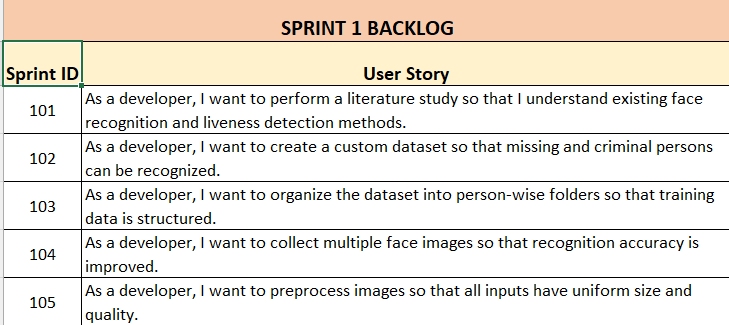
\includegraphics[width=12cm, height=8cm]{Sprint1.png}
	\caption{Sprint 1 Backlog}
	\label{fig:Sprint 1 Backlog}
\end{figure}
\begin{figure}[H]
	\centering
	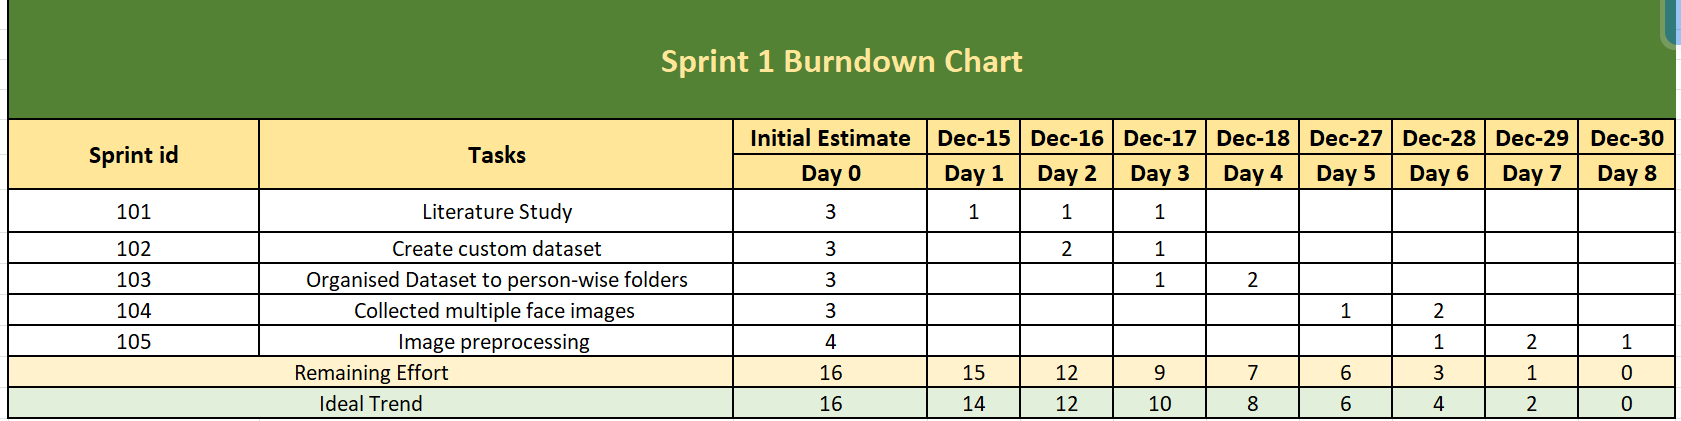
\includegraphics[width=16.5cm, height=8cm]{sprint1 burn.png}
	\caption{Sprint 1}
	\label{fig:Sprint 1}
\end{figure}
\begin{figure}[H]
	\centering
	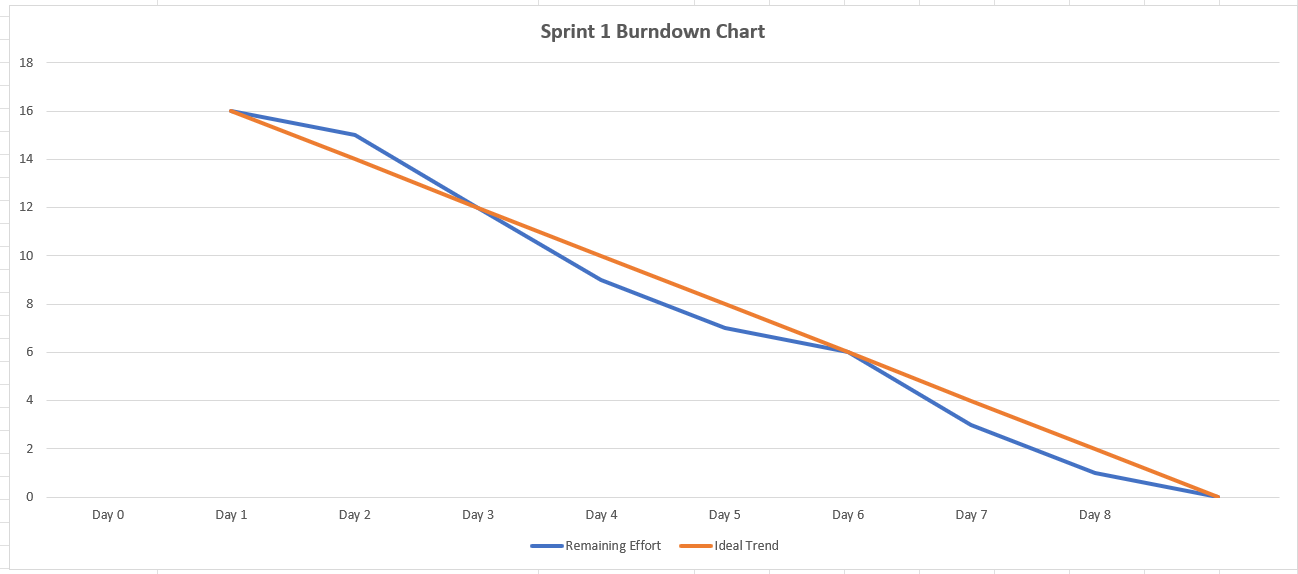
\includegraphics[width=16.5cm, height=8cm]{sprint1graph.png.png}
	\caption{Sprint 1 Burndown Chart}
	\label{fig:Sprint 1 Burndown chart}
\end{figure}
\begin{figure}[H]
	\centering
	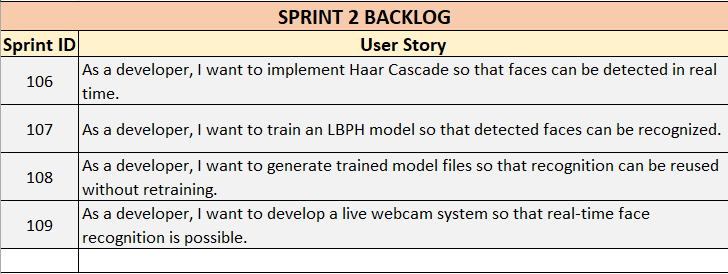
\includegraphics[width=16.5cm, height=8cm]{Sprint2Back.png}
	\caption{Sprint 2 Backlog}
	\label{fig:Sprint 2 Backlog}
\end{figure}
\begin{figure}[H]
	\centering
	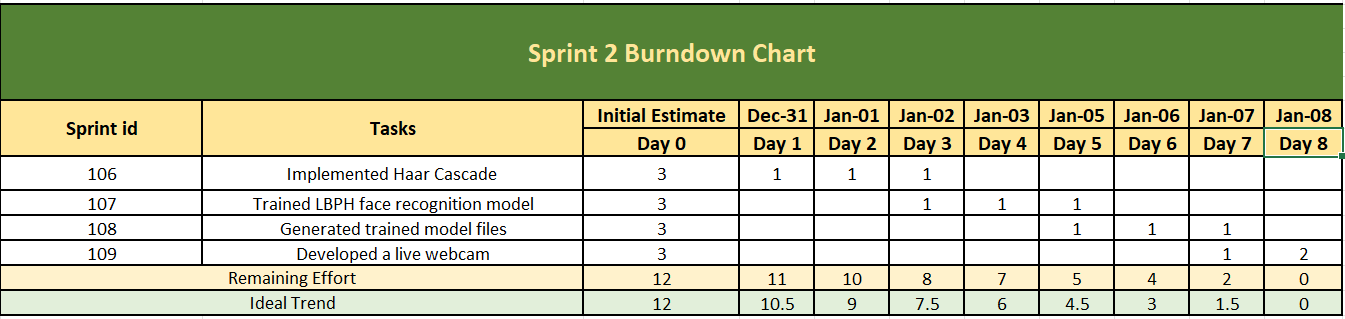
\includegraphics[width=16.5cm, height=8cm]{St2burn.png}
	\caption{Sprint 2}
	\label{fig:Sprint 2 }
\end{figure}
\begin{figure}[H]
	\centering
	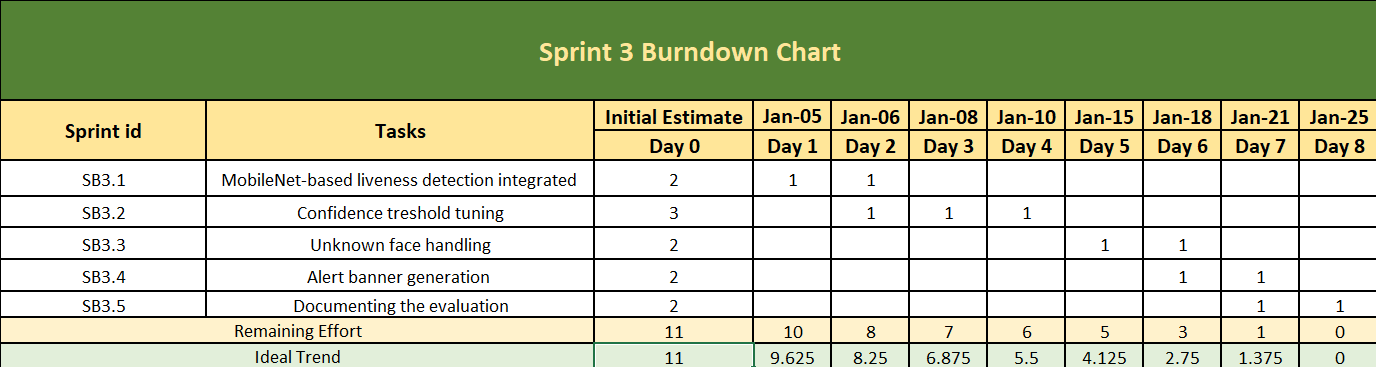
\includegraphics[width=16.5cm, height=8cm]{Spt3 burn.png}
	\caption{Sprint 3}
	\label{fig:Sprint 3 Burndown Chart  }
\end{figure}
\begin{figure}[H]
	\centering
	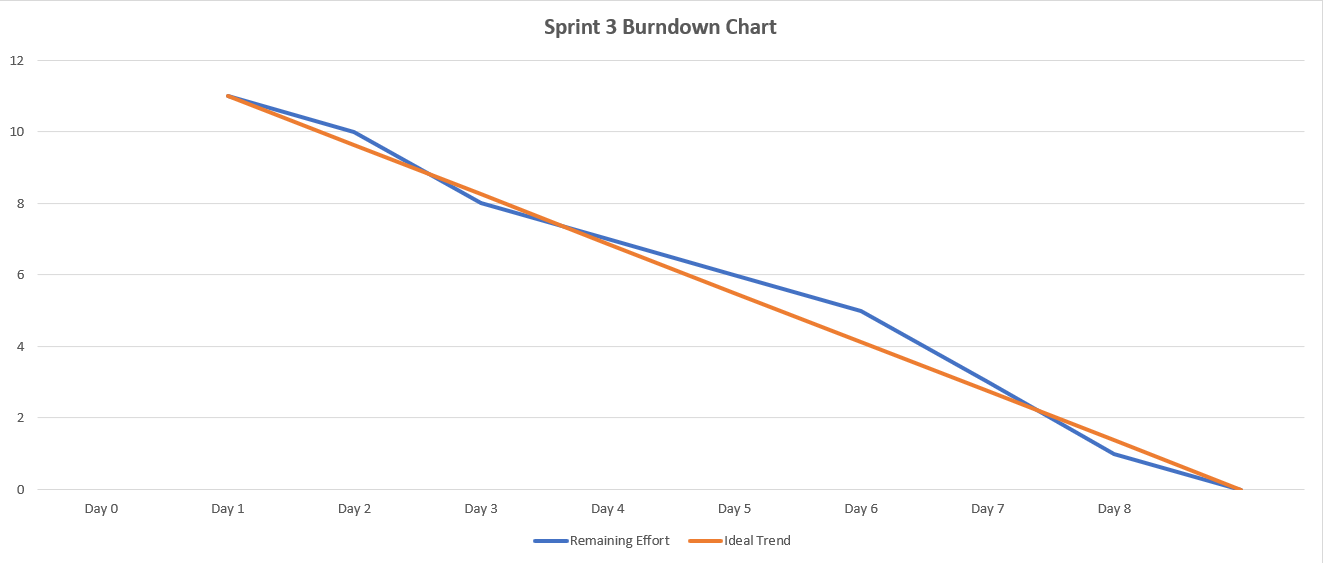
\includegraphics[width=16.5cm, height=8cm]{Spt3 chart.png}
	\caption{Sprint 3}
	\label{fig:Sprint 3 Burndown Chart  }
\end{figure}
\begin{figure}[H]
	\centering
	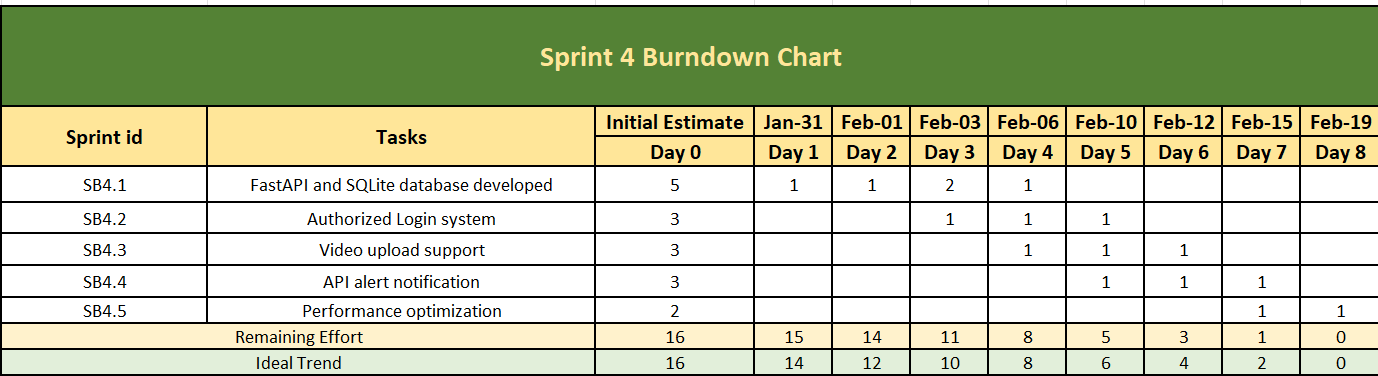
\includegraphics[width=16.5cm, height=8cm]{Spt4 burn.png} 
	\caption{Sprint 4}
	\label{fig:Sprint 4 Burndown Chart  }
\end{figure}
\begin{figure}[H]
	\centering
	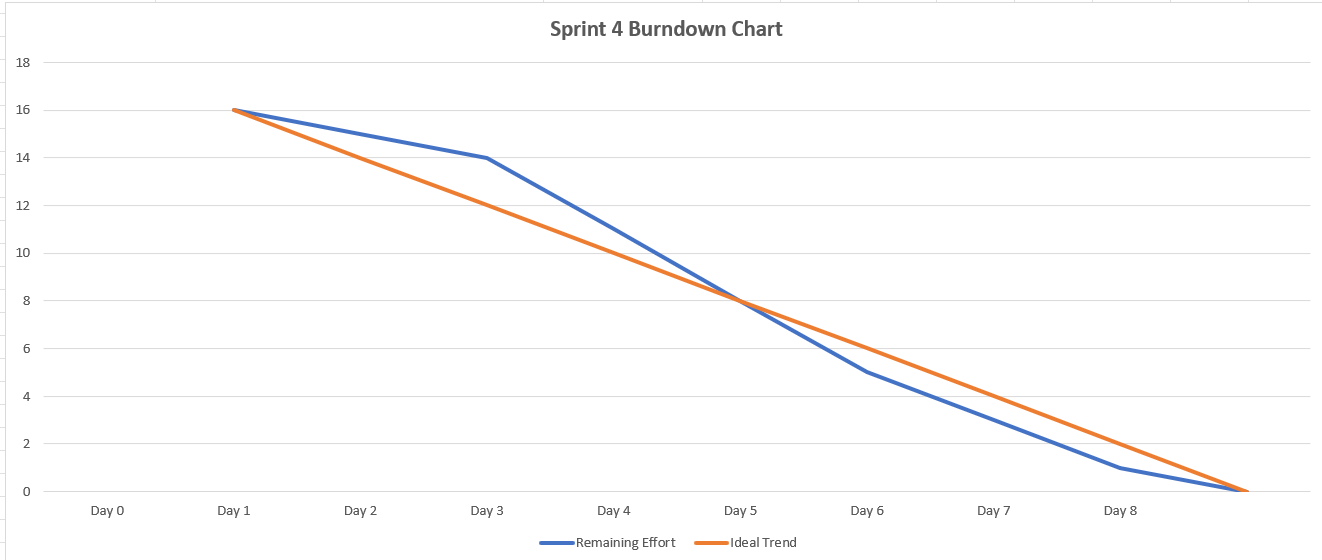
\includegraphics[width=16.5cm, height=8cm]{spt4 chart.png}
	\caption{Sprint 4}
	\label{fig:Sprint 4 Burndown Chart  }
\end{figure}
\section{Dataset}

Unlike traditional applications that rely on generic or unstructured data, the IDVision system uses a structured image dataset for face recognition. The dataset consists of labeled images of missing persons and criminal individuals, organized into separate folders for each person.

Each individual has a dedicated directory containing multiple face images captured under different conditions such as varying lighting, angles, and facial expressions. This diversity helps improve the robustness and accuracy of the recognition system. The dataset is further categorized into groups such as missing persons and criminals, enabling efficient classification and identification.

The dataset plays a crucial role in the system, as real-time detected faces are compared with the stored facial data to identify individuals accurately.
\section{Data Preprocessing}

Image data contains noise, variations in lighting, and inconsistencies in size and format. Two distinct preprocessing paths are therefore used in the system: one for offline training of the LBPH recogniser and one for online inference against the live webcam feed.

\textbf{Training-time preprocessing.} Every image under \texttt{dataset/\{criminals,\,missing\_persons\}/\{id\}\_\{Name\}/} is loaded with OpenCV and converted to grayscale. A Haar Cascade classifier (\texttt{haarcascade\_frontalface\_default.xml}) is then run over the grayscale frame; each detected face region is resized to a fixed $200\times200$ crop and appended to the training set with its integer label. Folder entries that are not directories, folder names that do not match the \texttt{\{id\}\_\{name\}} pattern, and images in which no face can be located are explicitly skipped and logged. Alongside the LBPH model, the trainer writes an enriched label map that records the folder, person id, name, and category (missing vs.\ criminal) for each label, so the recogniser no longer has to consult a separate JSON file for category lookup.

\textbf{Inference-time preprocessing.} On the live feed the Haar Cascade is replaced by OpenCV's YuNet detector, which is more robust to pose and illumination. For each detected face the bounding box is clamped to the frame, cropped, converted to grayscale, and resized to $200\times200$ before being passed to \texttt{LBPHFaceRecognizer.predict}. This matches the crop size used at training time, which is essential for LBPH to be comparable.
\section{Data Flow Diagram}

The Data Flow Diagram (DFD) illustrates the logical flow of information through the IDVision system, detailing how input data is processed into meaningful outputs such as identification results and alerts.

As shown in the figure below, the process begins at the login page of the Jinja2-rendered dashboard, where the user authenticates and then opens the live camera view. Authenticated HTTP requests drive the FastAPI backend, which reads frames from the webcam through OpenCV.

Each frame is passed into the processing pipeline, where YuNet (\texttt{FaceDetectorYN}) detects faces and returns bounding boxes. Each face region is cropped, grayscaled, resized to $200\times200$, and fed to the LBPH recogniser. The recogniser's output is filtered by a confidence threshold, resolved to a (name, category) pair through the enriched label map, and gated by a temporal streak filter that requires the same label to appear in 3 of the last 5 predictions before it is accepted as a match.

Once a match is accepted and the per-(name, category) cooldown permits, the alerting layer writes a row to the SQLite \texttt{alerts} table, appends a line to \texttt{alerts\_log.txt}, and dispatches an email over SMTP on a background thread. The alert carries the person's name, category, and timestamp.

The annotated frame (bounding box, label, confidence, colour-coded category) is encoded back to JPEG and streamed to the browser as an MJPEG feed, while the structured logs remain available through the dashboard's \emph{Recent detections} card and the alerts table.

\begin{figure}[H]
    \centering
    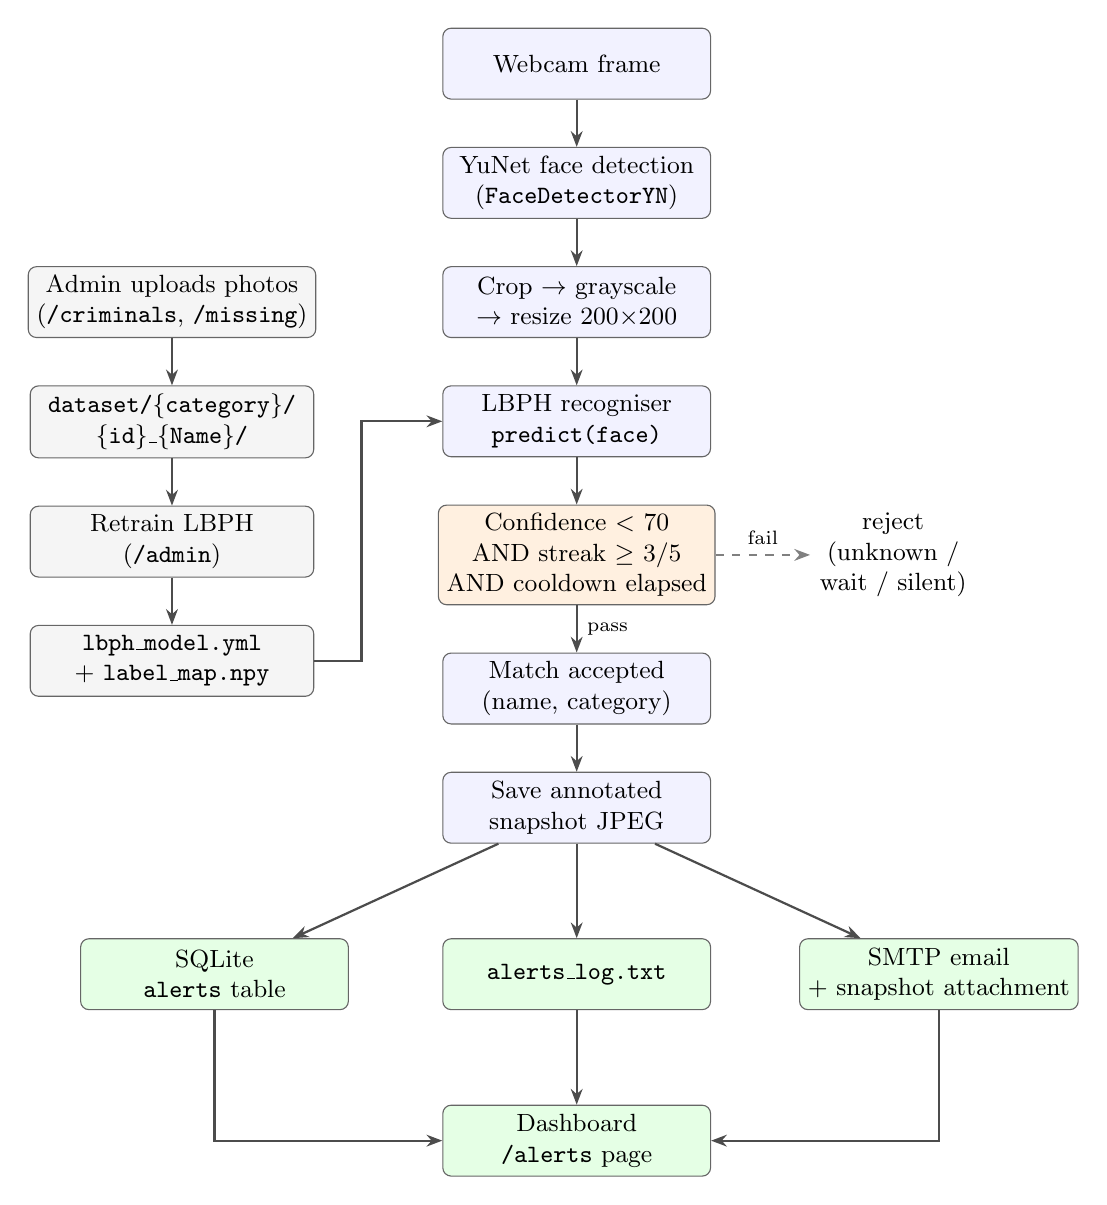
\begin{tikzpicture}[
        font=\small,
        node distance = 6mm and 10mm,
        every node/.style = {align=center},
        box/.style = {rectangle, rounded corners=3pt, draw=black!60,
                      fill=blue!5, minimum width=34mm, minimum height=9mm,
                      inner sep=3pt},
        gate/.style = {rectangle, rounded corners=3pt, draw=black!60,
                       fill=orange!12, minimum width=34mm, minimum height=9mm,
                       inner sep=3pt},
        sink/.style = {rectangle, rounded corners=3pt, draw=black!60,
                       fill=green!10, minimum width=34mm, minimum height=9mm,
                       inner sep=3pt},
        side/.style = {rectangle, rounded corners=3pt, draw=black!60,
                       fill=gray!8, minimum width=36mm, minimum height=9mm,
                       inner sep=3pt},
        arrow/.style = {-{Stealth[length=2mm]}, thick, draw=black!70},
        soft/.style  = {-{Stealth[length=2mm]}, thick, draw=black!50, dashed}
    ]

    % --- Main recognition pipeline (centre column, top to bottom) ---
    \node[box] (cam)   {Webcam frame};
    \node[box, below=of cam]  (det)  {YuNet face detection\\(\texttt{FaceDetectorYN})};
    \node[box, below=of det]  (prep) {Crop $\rightarrow$ grayscale\\$\rightarrow$ resize 200$\times$200};
    \node[box, below=of prep] (lbph) {LBPH recogniser\\\texttt{predict(face)}};
    \node[gate, below=of lbph] (gates) {Confidence $<$ 70 \\ AND streak $\geq$ 3/5 \\ AND cooldown elapsed};
    \node[box, below=of gates] (accept) {Match accepted\\(name, category)};
    \node[box, below=of accept] (snap)   {Save annotated\\snapshot JPEG};

    % --- Three alert sinks in a row ---
    \node[sink, below=12mm of snap, xshift=-46mm] (sqlite) {SQLite\\\texttt{alerts} table};
    \node[sink, below=12mm of snap]               (logf)   {\texttt{alerts\_log.txt}};
    \node[sink, below=12mm of snap, xshift=46mm]  (email)  {SMTP email\\+ snapshot attachment};

    % Dashboard sink
    \node[sink, below=12mm of logf] (dash) {Dashboard\\\texttt{/alerts} page};

    % --- Enrolment + training flow (left column) ---
    \node[side, left=16mm of prep] (upload) {Admin uploads photos\\(\texttt{/criminals}, \texttt{/missing})};
    \node[side, below=of upload]   (ds)     {\texttt{dataset/\{category\}/}\\\texttt{\{id\}\_\{Name\}/}};
    \node[side, below=of ds]       (train)  {Retrain LBPH\\(\texttt{/admin})};
    \node[side, below=of train]    (model)  {\texttt{lbph\_model.yml}\\+ \texttt{label\_map.npy}};

    % --- Main arrows ---
    \draw[arrow] (cam)    -- (det);
    \draw[arrow] (det)    -- (prep);
    \draw[arrow] (prep)   -- (lbph);
    \draw[arrow] (lbph)   -- (gates);
    \draw[arrow] (gates)  -- node[right, font=\scriptsize]{pass} (accept);
    \draw[arrow] (accept) -- (snap);
    \draw[arrow] (snap)   -- (sqlite);
    \draw[arrow] (snap)   -- (logf);
    \draw[arrow] (snap)   -- (email);
    \draw[arrow] (sqlite) |- (dash.west);
    \draw[arrow] (email)  |- (dash.east);
    \draw[arrow] (logf)   -- (dash);

    % --- Reject paths (dashed) ---
    \node[right=12mm of gates] (reject) {reject\\(unknown /\\wait / silent)};
    \draw[soft] (gates.east) -- node[above, font=\scriptsize]{fail} (reject.west);

    % --- Enrolment arrows and cross-link into recognition ---
    \draw[arrow] (upload) -- (ds);
    \draw[arrow] (ds)     -- (train);
    \draw[arrow] (train)  -- (model);
    \draw[arrow] (model.east) -- ++(6mm,0) |- (lbph.west);

    \end{tikzpicture}
    \caption{IDVision end-to-end workflow. Left column: admin enrolment and
    on-demand LBPH retraining. Centre column: per-frame recognition pipeline
    with the three gates (confidence threshold, temporal streak filter,
    per-(name,\,category) cooldown). Bottom row: three alert channels
    (SQLite, plain-text log, SMTP email with the snapshot JPEG attached),
    all visible through the dashboard's \texttt{/alerts} page.}
    \label{fig:project_workflow}
\end{figure}




\chapter{Architecture }  
\section{Model Architecture}

This chapter describes the architecture of the models used in the IDVision system and how they are combined into the live pipeline. The system is built around two OpenCV-based models and a set of rule-based gates:

\begin{itemize}
    \item Face Detection Model (YuNet, used in the live feed)
    \item Face Recognition Model (LBPH, trained on the custom dataset)
    \item Liveness Heuristic (Laplacian blur variance, standalone recogniser)
\end{itemize}

Each component is designed for a specific task and is invoked sequentially within the frame-by-frame pipeline.

\subsection{Face Detection Model (YuNet)}

Face detection in the live feed is performed by YuNet, a compact CNN-based face detector distributed as an ONNX file (\texttt{face\_detection\_yunet\_2023mar.onnx}) and loaded via OpenCV's \texttt{FaceDetectorYN.create}. Each frame is pushed through the detector at its native resolution (after \texttt{setInputSize}), producing a list of bounding boxes with confidence scores and five facial landmarks. YuNet replaces Haar Cascade in the live pipeline because it is markedly more robust to pose, lighting, and partial occlusion, which are common in surveillance scenarios. Haar Cascade is still used offline, but only as a crop tool during dataset preparation.

Key characteristics:
\begin{itemize}
    \item Single-shot CNN detector distributed as an ONNX model
    \item Tunable score and NMS thresholds (set to 0.9 and 0.3 in the code)
    \item Returns bounding box plus five facial landmarks per face
\end{itemize}

\subsection{Face Recognition Model (LBPH)}

Recognition is implemented using OpenCV's Local Binary Patterns Histograms recogniser (\texttt{cv2.face.LBPHFaceRecognizer\_create}). LBPH encodes each face as a spatially-gridded histogram of local binary patterns and performs nearest-neighbour matching in that histogram space; \texttt{predict} returns the nearest training label together with a distance value (lower is more similar).

The pipeline around LBPH in IDVision comprises three gates:
\begin{itemize}
    \item \textbf{Confidence threshold.} Any prediction whose distance is $\geq$ \texttt{LBPH\_CONFIDENCE\_THRESHOLD} (default 70) is treated as a no-match and fed into the streak buffer as a miss.
    \item \textbf{Label-to-category resolution.} Each trained label is resolved through an enriched \texttt{label\_map.npy} entry \texttt{\{folder, person\_id, name, category\}} that is written alongside the model at training time. Embedding the category directly in the label map eliminates the id-collision bug caused by criminals and missing\_persons sharing their auto-increment counters.
    \item \textbf{Streak filter.} A circular buffer of the last \texttt{RECOGNITION\_STREAK\_WINDOW} predictions (default 5) is maintained. A match is only accepted when the same label has appeared in at least \texttt{RECOGNITION\_STREAK\_REQUIRED} of those predictions (default 3). This suppresses the flickery singleton false positives that LBPH produces on small training sets.
\end{itemize}

\subsection{Liveness Heuristic (Laplacian Variance)}

A MobileNet-based liveness model was planned as part of the system design; in the shipped implementation liveness is approximated by a lightweight Laplacian-variance blur check retained in the standalone \texttt{live\_recognition\_haar.py} recogniser. The web application pipeline focuses on detection and recognition accuracy and treats proper CNN-based liveness as an explicit piece of future work (see Chapter~\ref{sec:future-work}).

\subsection{System Integration}

The overall live-feed architecture chains the following stages per frame:

\begin{enumerate}
    \item YuNet face detection (bounding boxes + landmarks)
    \item Crop, grayscale, resize to $200\times200$
    \item LBPH recognition + confidence threshold
    \item Per-label streak filter
    \item Per-(name, category) alert cooldown
    \item DB row + plain-text log + background-thread SMTP email
\end{enumerate}

An authenticated MJPEG stream returns annotated frames to the browser. The bounding-box label now also shows the raw LBPH confidence value so the threshold can be tuned from observed scores.

\section{Hyperparameter Details}

The system does not involve end-to-end deep-learning training. Its behaviour is nevertheless controlled by a set of parameters, all of which are env-configurable:

\textbf{YuNet Detector:}
\begin{itemize}
    \item Model: \texttt{face\_detection\_yunet\_2023mar.onnx}
    \item Input size: set per frame via \texttt{setInputSize}
    \item Score threshold: 0.9
    \item NMS threshold: 0.3
    \item Top-$k$: 5000
\end{itemize}

\textbf{LBPH Recogniser:}
\begin{itemize}
    \item Face crop: $200 \times 200$ grayscale
    \item \texttt{LBPH\_CONFIDENCE\_THRESHOLD}: 70 (lower = stricter)
    \item \texttt{RECOGNITION\_STREAK\_WINDOW}: 5 frames
    \item \texttt{RECOGNITION\_STREAK\_REQUIRED}: 3 of 5 to accept a match
    \item \texttt{ALERT\_COOLDOWN\_SECONDS}: 30 per (name, category)
\end{itemize}

\textbf{Liveness Heuristic:}
\begin{itemize}
    \item Metric: variance of the Laplacian of the grayscale face crop
    \item Threshold: 30 (values above $\Rightarrow$ treat as live)
\end{itemize}

\section{Performance Analysis}

The system performance is evaluated based on:

\begin{itemize}
    \item Recognition accuracy
    \item False acceptance and rejection rates
    \item Liveness detection accuracy
    \item Real-time processing efficiency
\end{itemize}

\begin{figure}[H]
    \centering
    \begin{tikzpicture}[
        font=\footnotesize,
        node distance = 5mm and 8mm,
        every node/.style = {align=center},
        io/.style    = {rectangle, rounded corners=3pt, draw=black!60,
                        fill=gray!8,  minimum width=38mm, minimum height=8.5mm,
                        inner sep=3pt},
        model/.style = {rectangle, rounded corners=3pt, draw=black!60,
                        fill=blue!8,  minimum width=38mm, minimum height=8.5mm,
                        inner sep=3pt},
        proc/.style  = {rectangle, rounded corners=3pt, draw=black!60,
                        fill=cyan!10, minimum width=38mm, minimum height=8.5mm,
                        inner sep=3pt},
        gate/.style  = {rectangle, rounded corners=3pt, draw=black!60,
                        fill=orange!15, minimum width=38mm, minimum height=8.5mm,
                        inner sep=3pt},
        out/.style   = {rectangle, rounded corners=3pt, draw=black!60,
                        fill=green!12, minimum width=38mm, minimum height=8.5mm,
                        inner sep=3pt},
        art/.style   = {rectangle, rounded corners=3pt, draw=black!60,
                        fill=yellow!15, minimum width=42mm, minimum height=8.5mm,
                        inner sep=3pt},
        arr/.style   = {-{Stealth[length=2mm]}, thick, draw=black!70},
        arrdash/.style = {-{Stealth[length=2mm]}, thick, draw=black!55, dashed},
        hdr/.style   = {font=\small\bfseries}
    ]

    % ---------- Training column (left) ----------
    \node[hdr] (thdr) {\textbf{Training (offline)}};
    \node[io,    below=of thdr]   (tin)   {Dataset images\\\texttt{dataset/\{cat\}/\{id\}\_\{Name\}/}};
    \node[proc,  below=of tin]    (tcrop) {Haar cascade face crop\\$\rightarrow$ grayscale $\rightarrow$ 200$\times$200};
    \node[model, below=of tcrop]  (ttrain){LBPH trainer\\\texttt{cv2.face.LBPHFaceRecognizer}};
    \node[art,   below=of ttrain] (tart)  {Artifacts:\\\texttt{lbph\_model.yml}\\\texttt{label\_map.npy}\\\texttt{persons.json}};

    % ---------- Inference column (right) ----------
    \node[hdr, right=50mm of thdr] (ihdr) {\textbf{Inference (per live frame)}};
    \node[io,   below=of ihdr] (iin) {Webcam BGR frame\\(H\,$\times$\,W\,$\times$\,3)};
    \node[model, below=of iin] (yn)  {\textbf{YuNet face detector} (ONNX CNN)\\score 0.9 · NMS 0.3 · top-k 5000};
    \node[io,    below=of yn]  (bb)  {Bounding boxes + landmarks};
    \node[proc,  below=of bb]  (prep){Crop $\rightarrow$ grayscale\\$\rightarrow$ resize 200$\times$200};
    \node[model, below=of prep](lbph){\textbf{LBPH recogniser}\\LBP histograms · NN in hist.\,space\\output: (label, distance)};
    \node[gate,  below=of lbph](conf){Confidence gate\\distance $<$ 70?};
    \node[proc,  below=of conf](lut) {Label $\rightarrow$ (name, category)\\via enriched label\_map};
    \node[gate,  below=of lut] (strk){Streak filter\\deque[5] · count(label) $\geq$ 3};
    \node[gate,  below=of strk](cool){Cooldown gate\\per (name, category), 30\,s};
    \node[out,   below=of cool](out) {Accepted match\\(name, category, confidence)};

    % ---------- Reject (side annotation) ----------
    \node[right=8mm of conf, align=left] (rej1) {\scriptsize no $\rightarrow$ mark miss};
    \draw[arrdash] (conf.east) -- (rej1.west);
    \node[right=8mm of strk, align=left] (rej2) {\scriptsize no $\rightarrow$ wait};
    \draw[arrdash] (strk.east) -- (rej2.west);
    \node[right=8mm of cool, align=left] (rej3) {\scriptsize no $\rightarrow$ silent};
    \draw[arrdash] (cool.east) -- (rej3.west);

    % ---------- Arrows (training) ----------
    \draw[arr] (tin)    -- (tcrop);
    \draw[arr] (tcrop)  -- (ttrain);
    \draw[arr] (ttrain) -- (tart);

    % ---------- Arrows (inference) ----------
    \draw[arr] (iin)  -- (yn);
    \draw[arr] (yn)   -- (bb);
    \draw[arr] (bb)   -- (prep);
    \draw[arr] (prep) -- (lbph);
    \draw[arr] (lbph) -- (conf);
    \draw[arr] (conf) -- node[right, font=\scriptsize]{pass} (lut);
    \draw[arr] (lut)  -- (strk);
    \draw[arr] (strk) -- node[right, font=\scriptsize]{pass} (cool);
    \draw[arr] (cool) -- node[right, font=\scriptsize]{pass} (out);

    % ---------- Cross-link: trained artifacts -> LBPH recogniser ----------
    \draw[arr] (tart.east) .. controls +(20mm,0) and +(-30mm,-8mm) .. (lbph.west)
          node[midway, above, sloped, font=\scriptsize]
          {model loaded at app startup / on \texttt{/retrain}};

    \end{tikzpicture}
    \caption{IDVision model architecture. The left column shows the offline
    training pipeline (Haar cascade cropping feeds LBPH's trainer and
    produces the three model artifacts). The right column shows the
    per-frame inference stack — YuNet ONNX detection, preprocessing to the
    $200\times200$ grayscale crop LBPH expects, LBPH histogram matching,
    and the three gates (confidence threshold, temporal streak filter,
    per-(name,\,category) cooldown) that together produce an accepted
    match. Dashed arrows mark the reject branches. The trained artifacts
    are consumed by the inference recogniser at application startup and
    after every \texttt{/retrain}.}
    \label{fig:model-architecture}
\end{figure}

\subsection{User Input and Video Capture}
The user signs in through a Jinja2-rendered login page and the dashboard exposes the live camera as an MJPEG stream at \texttt{/video\_feed}. The frontend consists of server-rendered HTML templates with a shared dark-theme inline CSS; no SPA framework, build step, or separate JavaScript bundle is required. Protected routes (\texttt{/dashboard}, \texttt{/video\_feed}, \texttt{/criminals/add}, \texttt{/missing/add}, \texttt{/retrain}) redirect anonymous users to the login page.

\subsection{Backend Processing (Face Detection and Preprocessing)}
The backend is a FastAPI application organised into a small \texttt{idvision} package (\texttt{config}, \texttt{db}, \texttt{recognition}, \texttt{camera}, \texttt{enrollment}, \texttt{training}, \texttt{notifications}, \texttt{utils}, \texttt{deps}, and \texttt{routes/}). The camera module opens the webcam once at startup via \texttt{cv2.VideoCapture} and yields annotated JPEG frames to the video endpoint.

Key operations per frame:
\begin{itemize}
    \item Read next frame from the webcam
    \item Run YuNet (\texttt{FaceDetectorYN}) to obtain bounding boxes
    \item For each bounding box: clamp to frame, crop, convert to grayscale, resize to $200\times200$
    \item Feed the crop to the LBPH recogniser
    \item Annotate the frame with a coloured box and label that includes the raw LBPH confidence
    \item Encode the frame back to JPEG and yield it to the HTTP stream
\end{itemize}

\subsection{Liveness Heuristic}
A MobileNet-based liveness model was originally planned as part of the pipeline. The shipped system retains a lightweight Laplacian-variance check in the standalone \texttt{live\_recognition\_haar.py} recogniser as a placeholder, with a CNN-based liveness model called out as the highest-priority item in the future-work list. The web pipeline itself therefore delegates spoof resistance to the other gates (threshold, streak filter, operator in-loop review of the dashboard).

\subsection{Face Recognition and Identification}
Recognition uses OpenCV's LBPH recogniser (\texttt{cv2.face.LBPHFaceRecognizer}). Each face crop is passed to \texttt{predict}, which returns a label and a distance. The \texttt{FaceRecognizer} wrapper then applies three gates before exposing a match to the alerting layer: a confidence threshold, a category-aware label-map lookup (so \texttt{1\_Riya} in \texttt{missing\_persons/} and \texttt{1\_yaseen} in \texttt{criminals/} cannot collide on person id), and a temporal streak filter that requires the same label to appear in at least 3 of the last 5 predictions.


\subsection{Alert Generation and Analysis}
When recognition returns a match that passes the confidence and streak gates, the alerting layer writes the event through three channels: a row in the SQLite \texttt{alerts} table, a line appended to \texttt{alerts\_log.txt}, and an SMTP email dispatched on a background daemon thread so mail latency never stalls the camera. A per-(name, category) cooldown (default 30 seconds) gates all three channels, so a long continuous detection does not flood the inbox or the log.

Each alert carries:
\begin{itemize}
    \item Identified person name
    \item Category (missing person or criminal)
    \item Timestamp of detection
\end{itemize}

SMTP parameters (host, port, sender, app password, recipient list) are supplied via \texttt{.env}. If email is not configured, the DB and file log channels still fire; if SMTP is configured but fails at send time, the error is logged but does not disrupt recognition.

\subsection*{Key Outputs}

Key outputs include:
\begin{itemize}
    \item Identified person name
    \item Category (missing person or criminal)
    \item Timestamp of detection
\end{itemize}

The system ensures that alerts are generated efficiently while avoiding redundant notifications.

\subsection{ Result Visualization}

The processed results are returned to the frontend through the FastAPI-based REST API. The frontend displays the detected faces, identification results, and alerts in a structured format for the user.

This allows real-time monitoring and quick decision-making.

\subsection{ Data Storage and History Tracking}

The system uses SQLite for persistent storage. It stores:
\begin{itemize}
    \item Detected person details
    \item Alert logs
    \item Timestamp and detection history
\end{itemize}

This enables users to review past detections and maintain records for analysis.

\subsection{Conclusion}

The \textit{IDVision} architecture integrates FastAPI, OpenCV (with contrib modules), YuNet for detection and LBPH for recognition to create an efficient, explainable surveillance system. By combining a deep face detector with a classical recogniser stabilised by a temporal streak filter, and by gating alerts through a cooldown and SMTP dispatch, the system provides reliable, non-redundant real-time identification, with all configuration surfaced through \texttt{.env} rather than hard-coded.
\chapter{Results \& Explainability of the System }  
\section{Results}

The \textit{IDVision} system was evaluated using multiple video inputs and real-time camera streams to assess its ability to accurately detect, verify, and recognize individuals. The system successfully processed input data and generated identification results and alerts in real time.

The key results obtained include:

\begin{itemize}
    \item \textbf{Face Detection:} YuNet detects faces reliably in the live webcam stream across the lighting and pose conditions tested during demos, with the raw confidence values visible on every bounding box for transparency.

    \item \textbf{Recognition Accuracy:} The LBPH recogniser correctly identifies enrolled individuals from the dataset. Accuracy is sensitive to the size and variety of training images; false positives observed with a small training set are suppressed by the streak filter, which requires three agreeing predictions in a five-frame window before firing an alert.

    \item \textbf{Liveness Heuristic:} The Laplacian-variance check acts as a basic sharpness gate in the standalone recogniser; a CNN-based liveness model is an explicit piece of future work.

    \item \textbf{Real-Time Alert Generation:} Matches are written to the SQLite \texttt{alerts} table, appended to \texttt{alerts\_log.txt}, and emailed to configured recipients over SMTP STARTTLS on a background thread. All three channels are gated by a per-(name, category) cooldown.
\end{itemize}

The system demonstrates efficient real-time performance and reliable identification across different scenarios. The results are presented through:

\begin{itemize}
    \item Detection and recognition output displayed on the user interface
    \item Alert logs showing identified individuals and timestamps
    \item Structured visualization of results for easy monitoring
\end{itemize}

The evaluation shows that the system provides consistent and accurate results, making it suitable for real-time surveillance applications.

\section{Explainability of the System}

The \textit{IDVision} system incorporates partial explainability through transparent processing steps and interpretable decision-making mechanisms.

The explainability is achieved through the following components:

\begin{itemize}
    \item \textbf{Detection Transparency:} The system visually highlights detected faces with a bounding box so the operator can see exactly which regions are being processed.

    \item \textbf{Confidence on Screen:} The LBPH confidence value (a distance, where lower = better match) is drawn onto the bounding-box label of every recognised face, making the recogniser's certainty directly observable rather than hidden behind a thresholded boolean.

    \item \textbf{Colour-Coded Categories:} Box colour encodes the decision (red for criminal, orange for missing, yellow for known-unknown, green for detect-only), so the outcome is communicated at a glance.

    \item \textbf{Recognition Logic:} The LBPH histogram-distance formulation is mathematically interpretable, and the streak filter is a transparent rule (``appear in $K$ of the last $N$'') rather than an opaque learned gate.

    \item \textbf{Result Visibility:} Every alert's name, category, and timestamp is shown on the dashboard's \emph{Recent detections} card and is also persisted to the SQLite log, so users can audit detection history.
\end{itemize}

Although the system does not use advanced Explainable AI techniques such as SHAP or LIME, it provides a level of interpretability through its structured pipeline and transparent processing steps.
\section*{Discussion}

The integration of computer vision techniques with deep learning models provides a balance between accuracy and interpretability. Each stage of the system—from face detection to liveness verification and recognition—is structured and explainable.

This makes the system suitable for real-world surveillance applications, where both reliability and transparency are essential.

However, the system may have limitations under challenging conditions such as poor lighting, extreme facial angles, or occlusions, which can affect detection and recognition accuracy. Additionally, liveness detection performance may vary depending on environmental factors and input quality.

Despite these limitations, the system demonstrates strong potential for enhancing security through automated and intelligent surveillance.


\chapter{Conclusion}

\section{Summary}

The \textit{IDVision} system presents an efficient and intelligent solution for real-time surveillance using a combination of deep face detection and classical face recognition. The system successfully detects and recognises individuals from the live webcam stream and surfaces them through a role-based web dashboard.

By integrating YuNet for live face detection, Haar Cascade for training-time face cropping, and LBPH for face recognition, the system balances accuracy with explainability. A per-label streak filter is applied on top of LBPH to suppress the flickery false positives characteristic of small training sets, and a per-(name, category) cooldown gate protects the alert channels (SQLite, plain-text log, and SMTP email) from flooding.

The implementation uses a FastAPI backend with bcrypt-hashed passwords, signed session cookies, role-based access control, and magic-byte-validated photo uploads. An admin-only dashboard enables enrolment and in-process retraining of the LBPH model without a command-line round-trip. All configuration (session secret, database path, SMTP credentials, recognition thresholds, upload size) is loaded from a \texttt{.env} file so no secrets are hard-coded in the repository.

Overall, the system achieves its objective of providing automated, accurate, and real-time identification of individuals, reducing human effort and improving surveillance efficiency.

\subsection{Future Work}\label{sec:future-work}

Although the current system performs effectively, several enhancements can be considered to improve its capabilities and scalability:

\begin{itemize}
    \item \textbf{Deep-Embedding Recogniser:} Replace LBPH with a deep face-embedding model such as FaceNet, ArcFace, or dlib's 128-dimensional ResNet embedding, and perform cosine-similarity matching against enrolled embeddings. This is the highest-impact accuracy upgrade and the natural path for removing the current false-positive sensitivity on small datasets.

    \item \textbf{CNN-Based Liveness:} Ship a properly trained MobileNet (or similar) liveness head in place of the Laplacian-variance placeholder, and invoke it in the web pipeline (not just the standalone recogniser).

    \item \textbf{Detection Upgrade:} Consider RetinaFace or a YOLO-family detector if YuNet's performance proves insufficient on harder scenes.

    \item \textbf{Multi-Camera Integration:} Extend the camera module from a single \texttt{cv2.VideoCapture} instance to a multiplexed pool of sources, with per-camera labels threaded through alerts.

    \item \textbf{Mobile Application:} Build a thin mobile client that reads the alerts feed over HTTPS and sends push notifications instead of only SMTP email.

    \item \textbf{GPS Location Integration:} Attach a camera location (fixed or GPS-provided) to every alert payload so downstream systems know where a subject was spotted.

    \item \textbf{Image Proof Generation:} Save the cropped face region of every alert to disk and attach it to the email body so recipients see visual evidence alongside the text.

    \item \textbf{CSRF Protection:} Add a CSRF token flow to mutating forms; the current \texttt{SameSite=Lax} session cookie is adequate for a demo but not production.

    \item \textbf{Automated Retrain on Enrol:} Trigger an asynchronous \texttt{train()} call after a successful photo upload so the admin no longer has to press \emph{Retrain} manually.
\end{itemize}

In conclusion, \textit{IDVision} provides a scalable, efficient, and user-friendly surveillance solution by combining computer vision techniques with deep learning-based recognition. The project demonstrates the effectiveness of automated systems in enhancing security and enabling real-time decision-making, making it suitable for modern surveillance applications.

%%%%%%%%%%%%%%%%%%%% BIBLIOGRAPHY %%%%%%%%%%%%%%%%%%%%

\begin{thebibliography}{99}

\bibitem{ref1}
C.-H. Yeh and H.-H. Chang, “Face liveness detection with feature discrimination between sharpness and blurriness,” 2017.

\bibitem{ref2}
A. Prasad and Anuradha, “Face anti-spoofing and liveliness detection using MobileNet and Haar Cascade,” 2025.

\bibitem{ref3}
J. Deng, J. Guo, Y. Zhou, J. Yu, I. Kotsia, and S. Zafeiriou, “RetinaFace: Single-shot multi-level face localisation in the wild.”

\bibitem{ref4}
H. Xing, S. Y. Tan, F. Qamar, and Y. Jiao, “Face anti-spoofing based on deep learning: A comprehensive survey,” 2025.

\bibitem{ref5}
“FastAPI documentation,” 2024. [Online]. Available: https://fastapi.tiangolo.com

\bibitem{ref6}
“SQLite documentation,” 2024. [Online]. Available: https://www.sqlite.org/docs.html
\end{thebibliography}
\chapter{Appendix}

\begin{figure}[H]
    \centering
    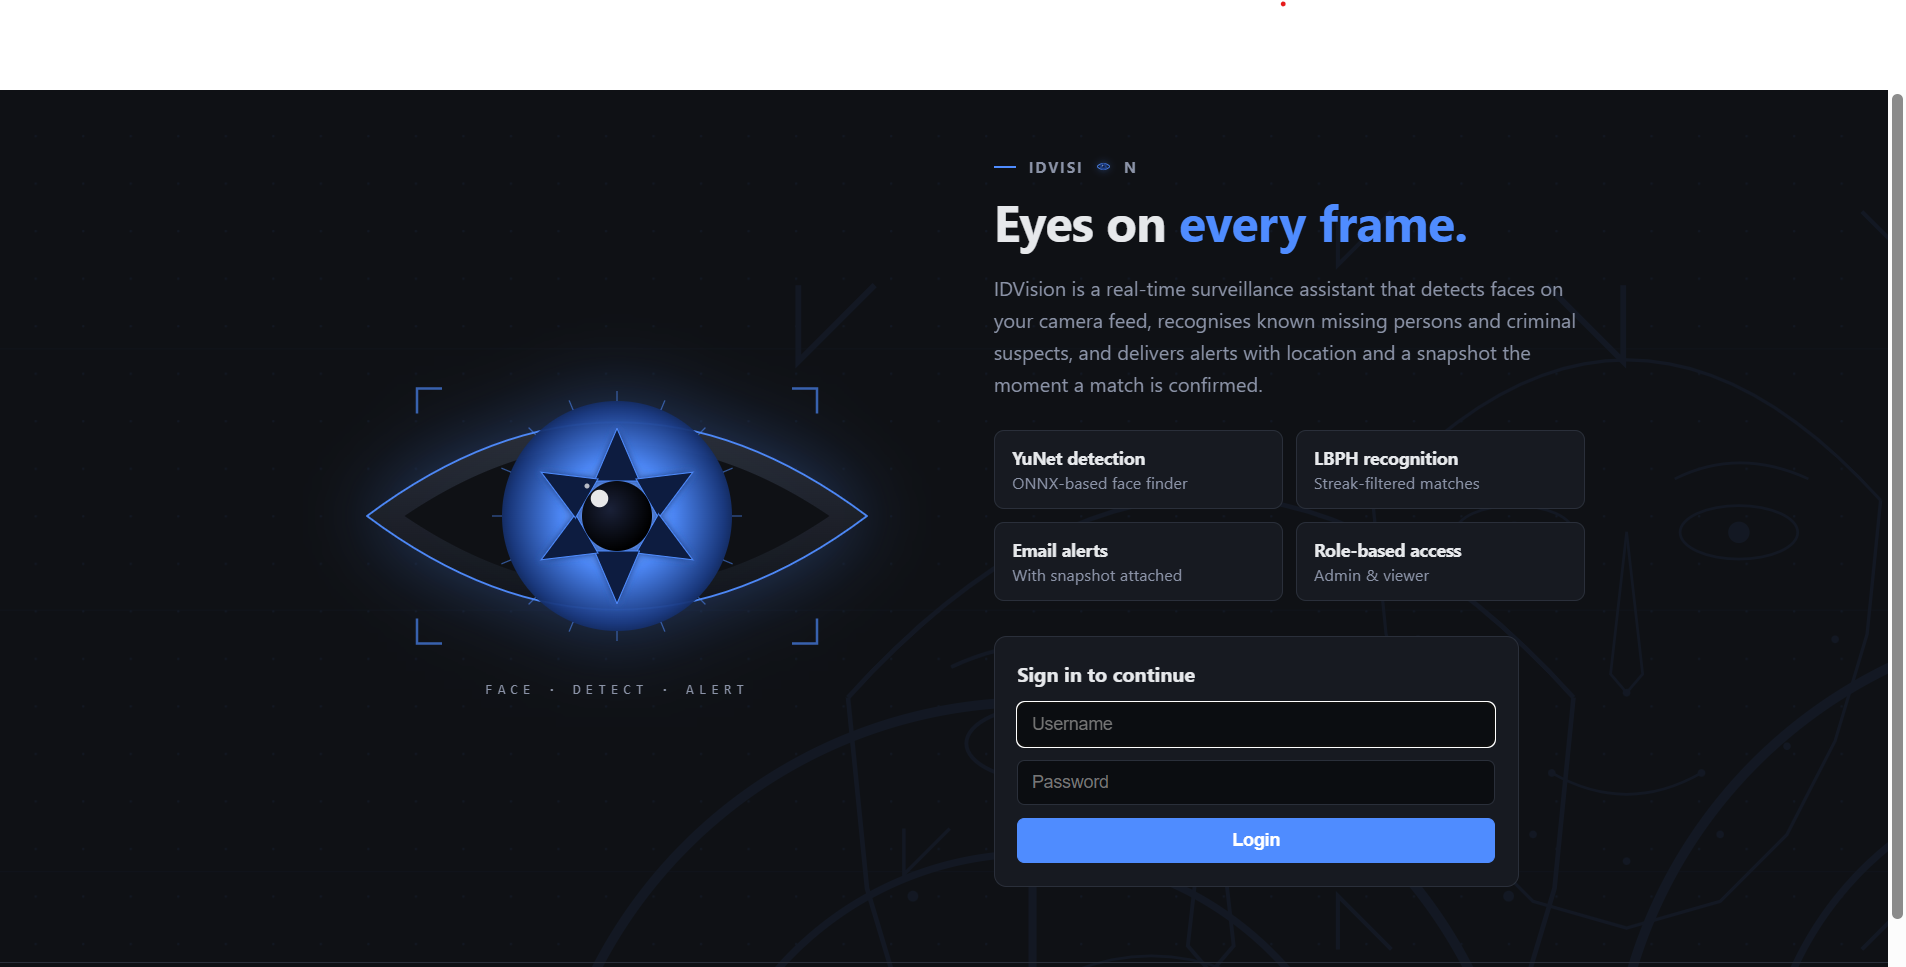
\includegraphics[width=0.85\linewidth]{home.png}
    \caption{Landing page (\texttt{/}) with the eye-camera hero illustration and the login form.}
    \label{fig:ui-home}
\end{figure}

\begin{figure}[H]
    \centering
    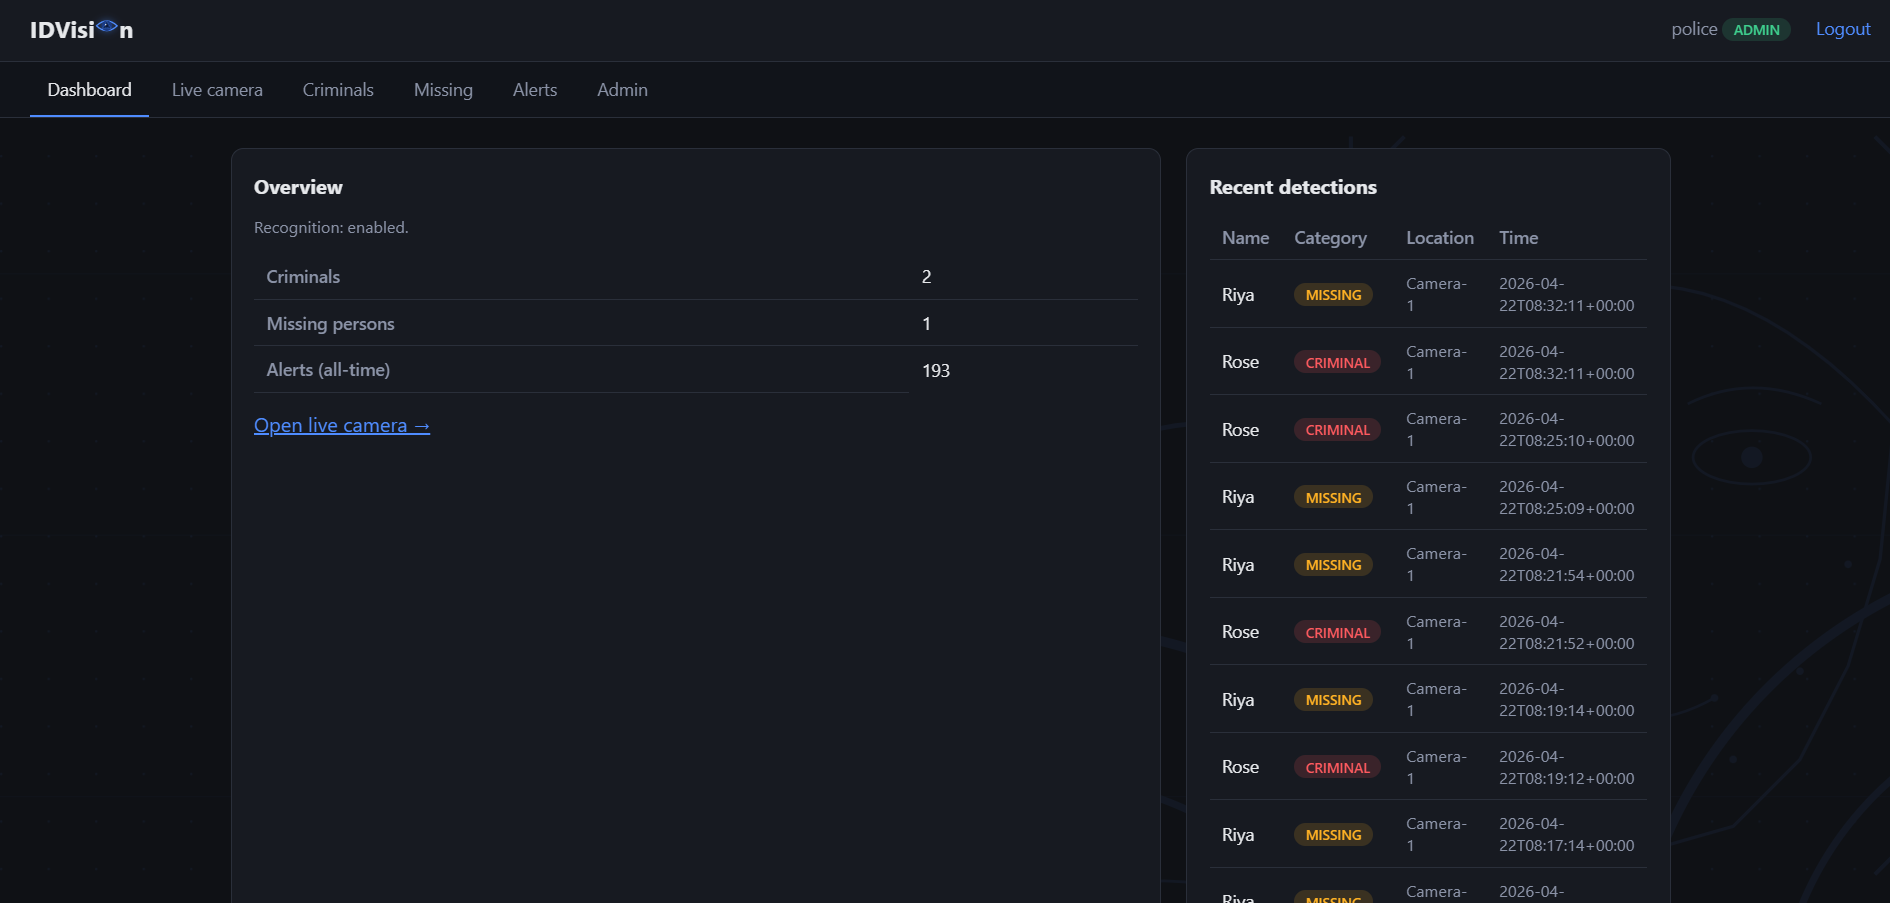
\includegraphics[width=0.85\linewidth]{dashboard.png}
    \caption{Dashboard (\texttt{/dashboard}) with the overview stats panel and recent-detections card.}
    \label{fig:ui-dashboard}
\end{figure}

\begin{figure}[H]
    \centering
    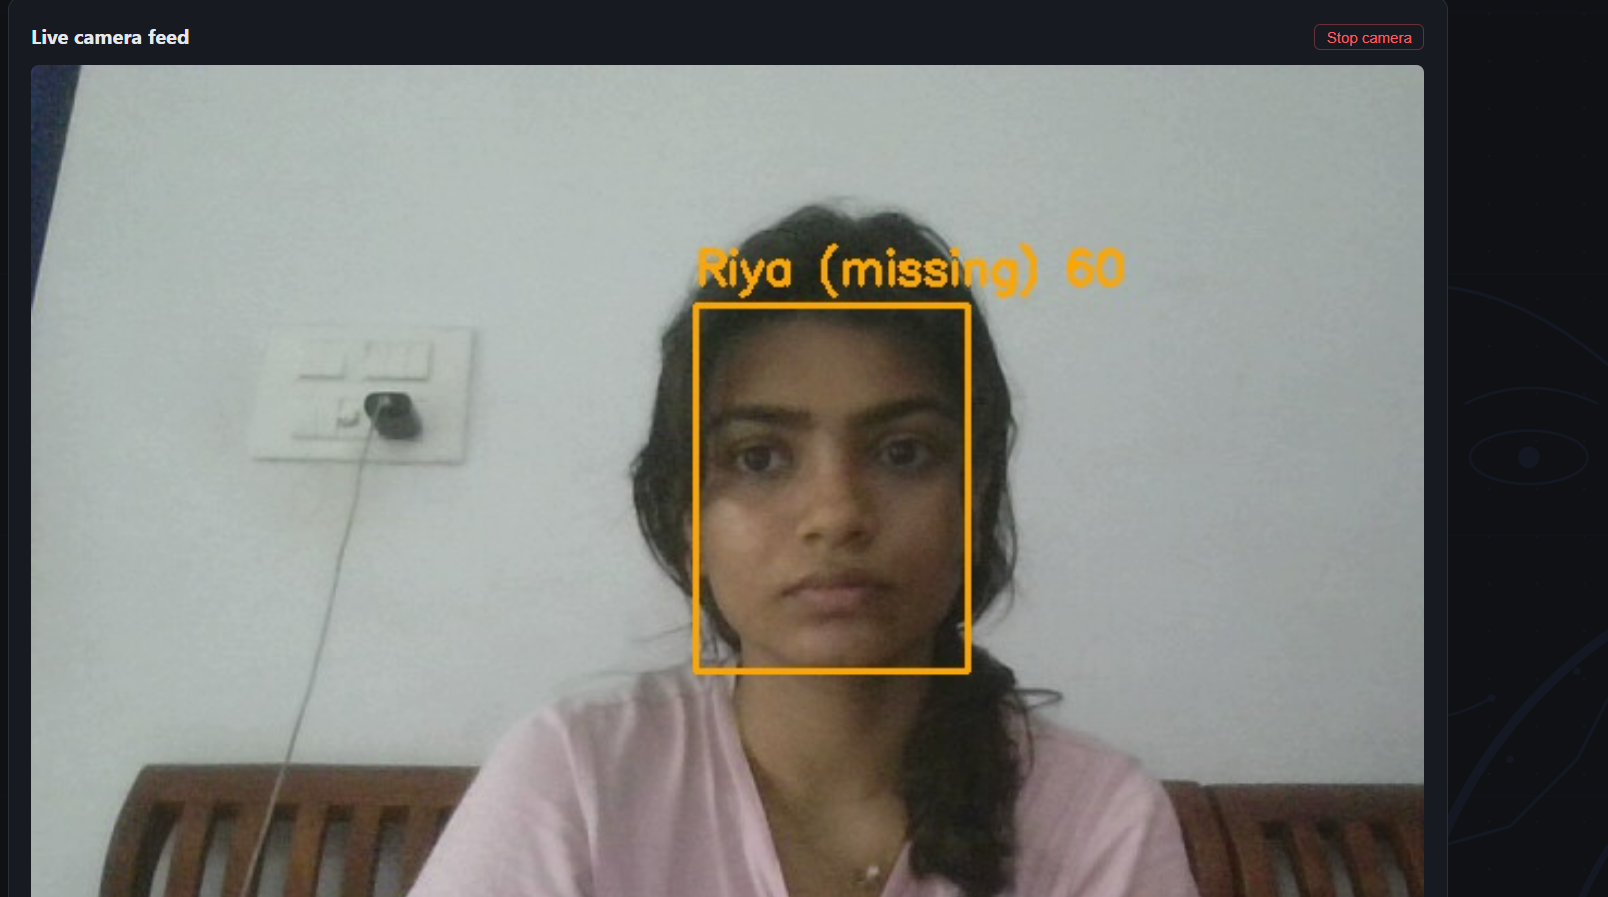
\includegraphics[width=0.85\linewidth]{camera.png}
    \caption{Live camera page (\texttt{/camera}) showing the annotated MJPEG feed and the Start/Stop control.}
    \label{fig:ui-camera}
\end{figure}

\begin{figure}[H]
    \centering
    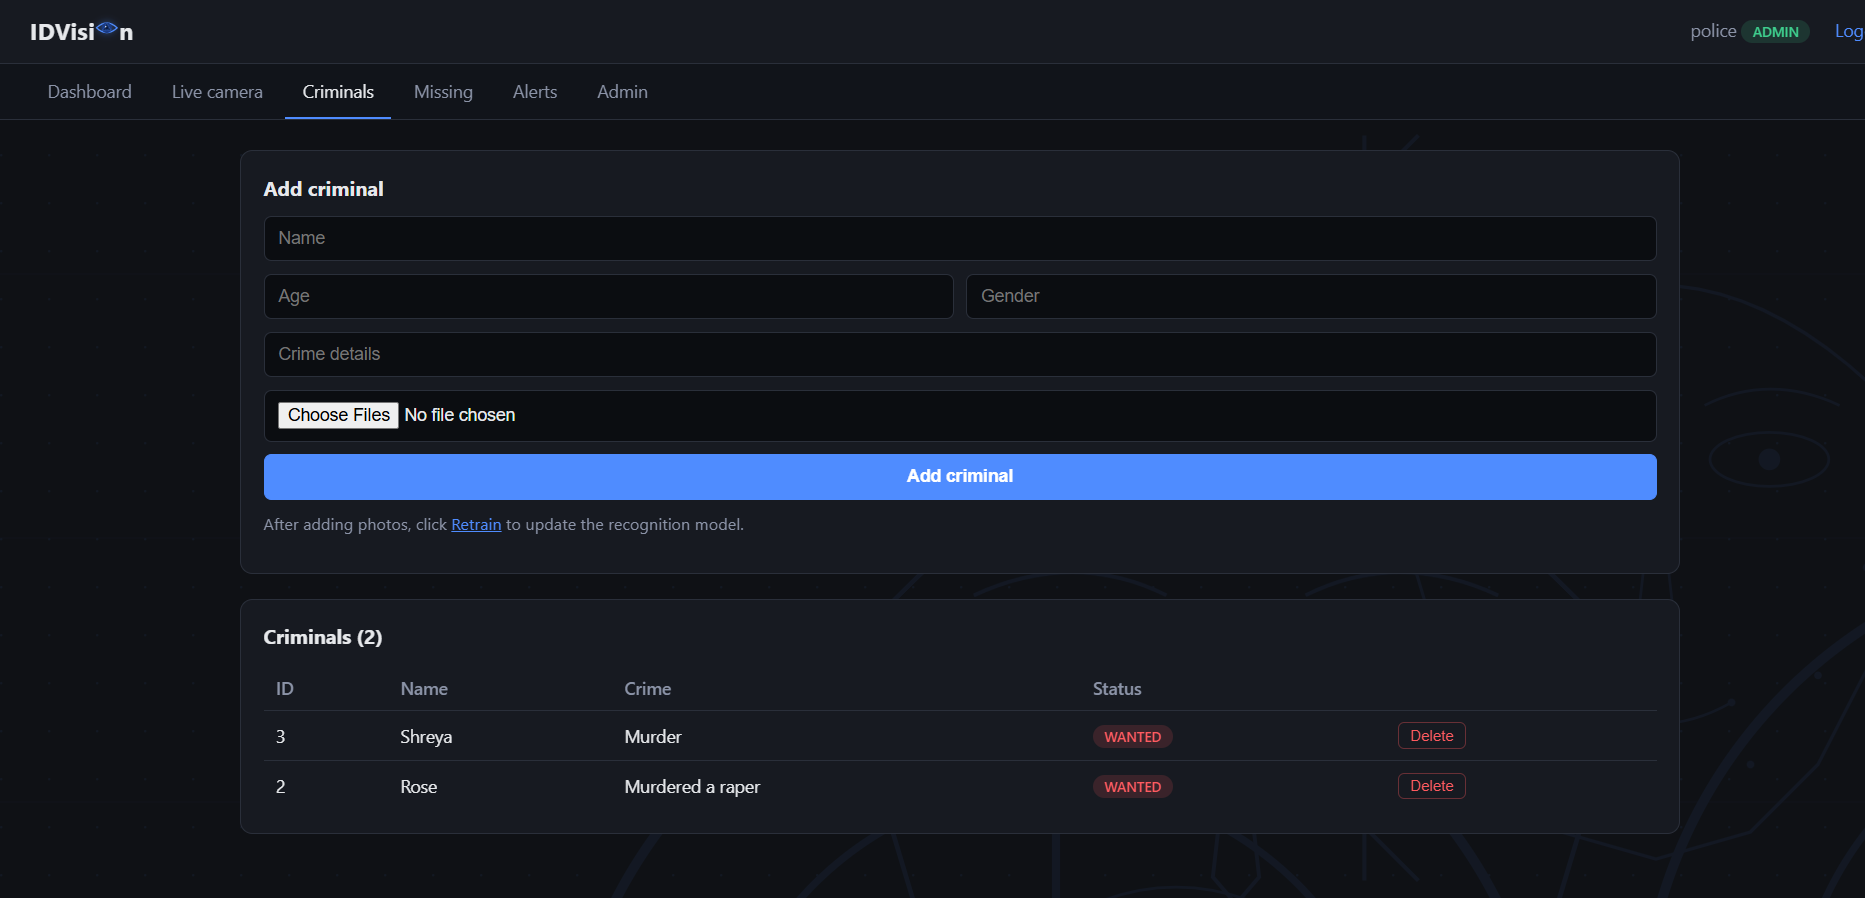
\includegraphics[width=0.85\linewidth]{criminals.png}
    \caption{Criminals page (\texttt{/criminals}) with the admin-only add form and the list of existing entries.}
    \label{fig:ui-criminals}
\end{figure}

\begin{figure}[H]
    \centering
    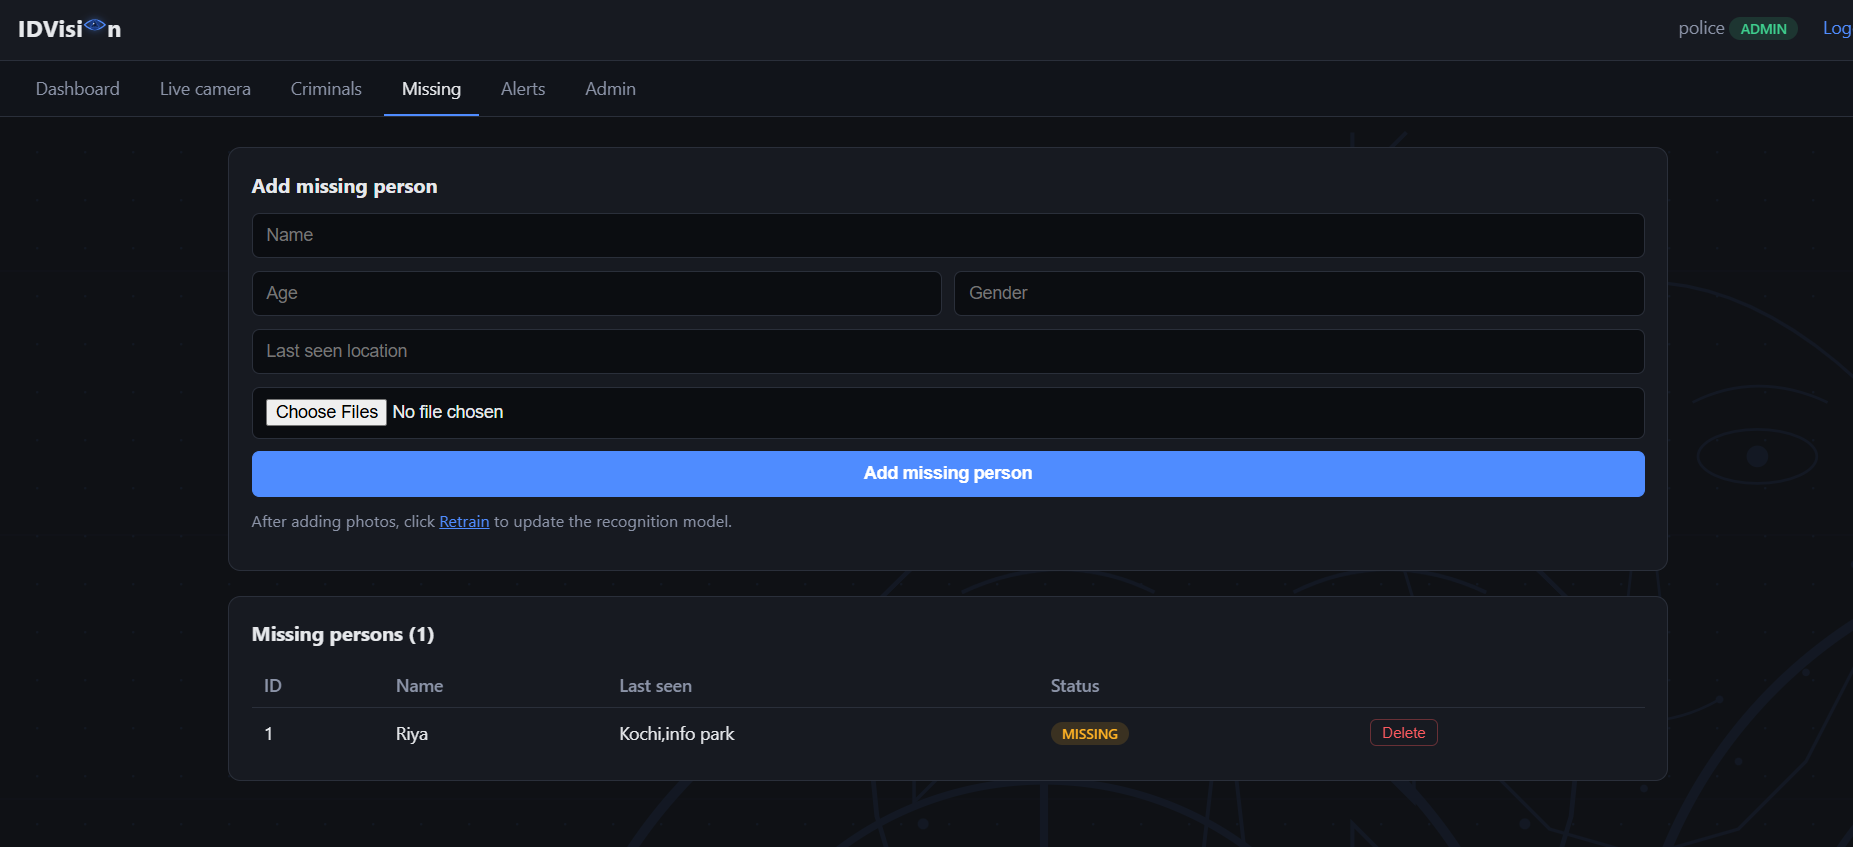
\includegraphics[width=0.85\linewidth]{missing.png}
    \caption{Missing persons page (\texttt{/missing}) with the add form and list.}
    \label{fig:ui-missing}
\end{figure}

\begin{figure}[H]
    \centering
    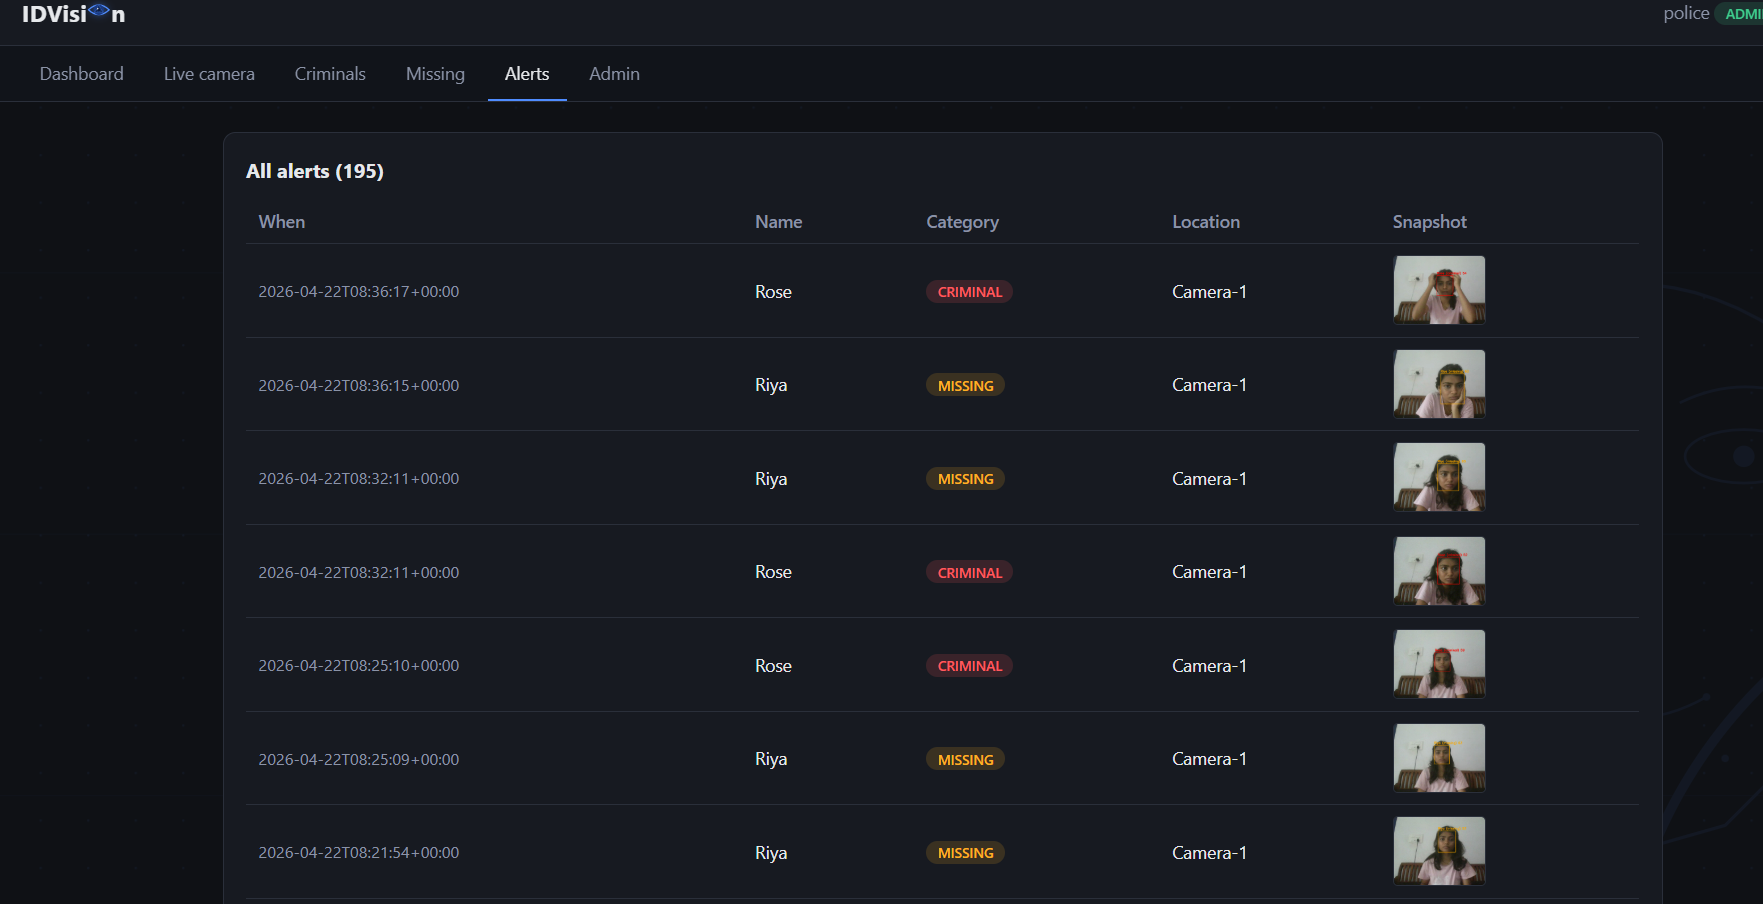
\includegraphics[width=0.85\linewidth]{alerts.png}
    \caption{Alerts page (\texttt{/alerts}) with inline snapshot thumbnails, location, and timestamps.}
    \label{fig:ui-alerts}
\end{figure}

\begin{figure}[H]
    \centering
    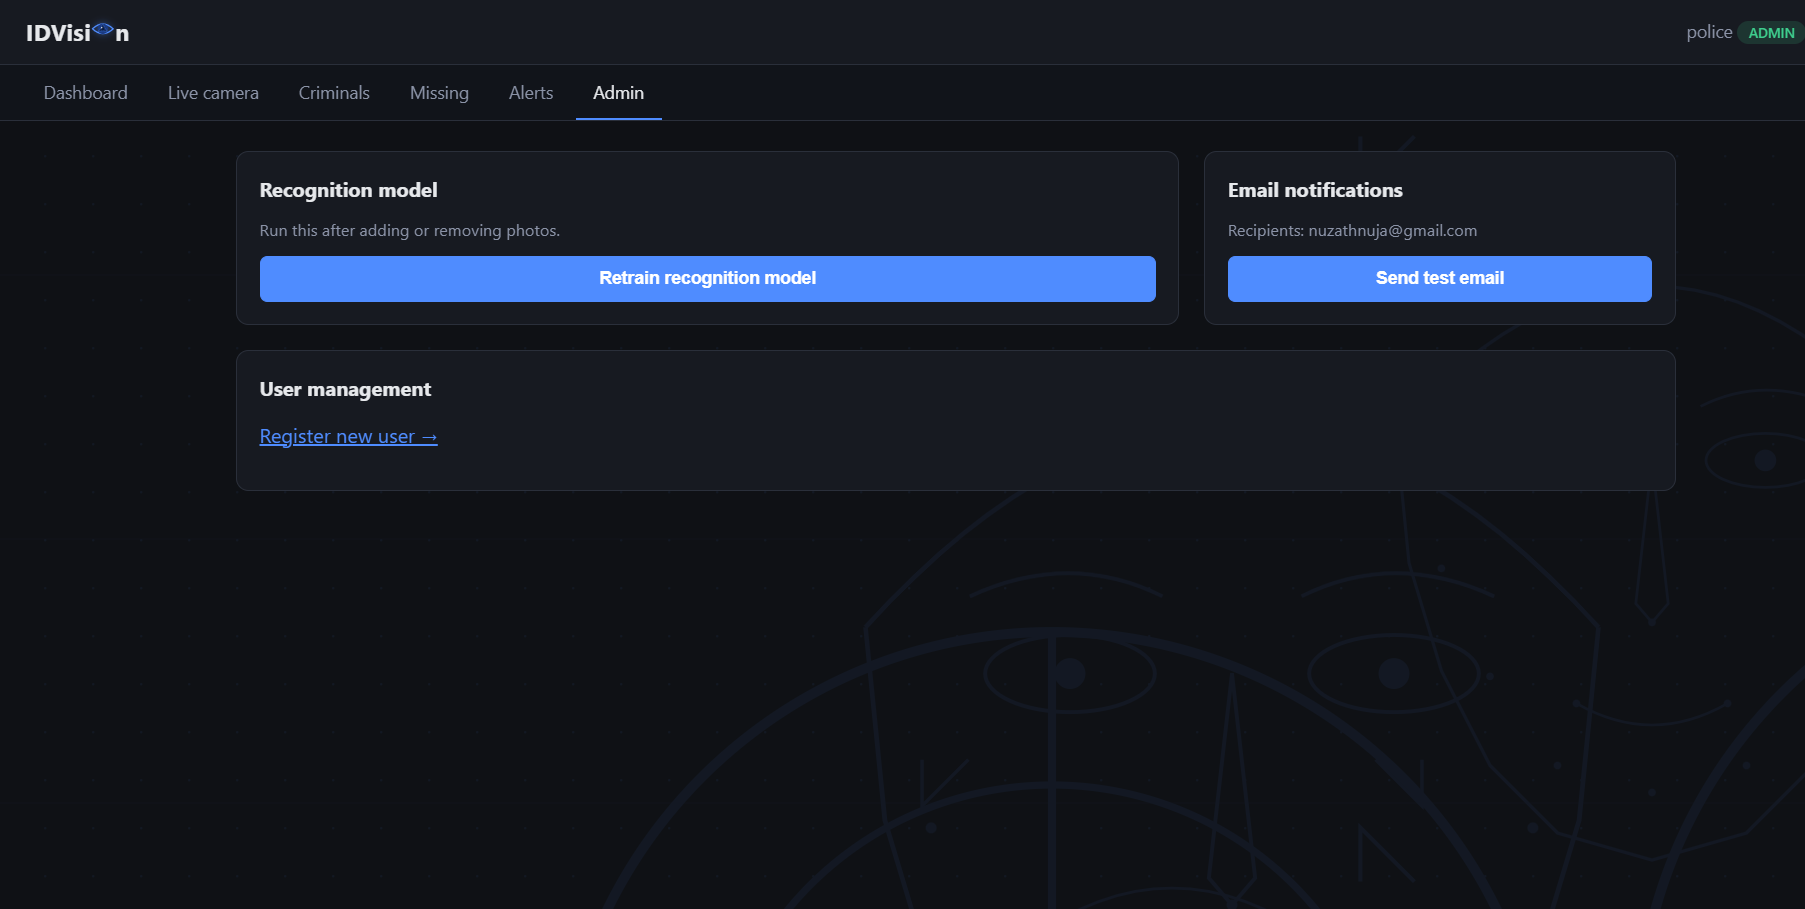
\includegraphics[width=0.85\linewidth]{admin.png}
    \caption{Admin page (\texttt{/admin}) — retrain the recognition model, send a test email, register new users.}
    \label{fig:ui-admin}
\end{figure}

\begin{figure}[H]
    \centering
    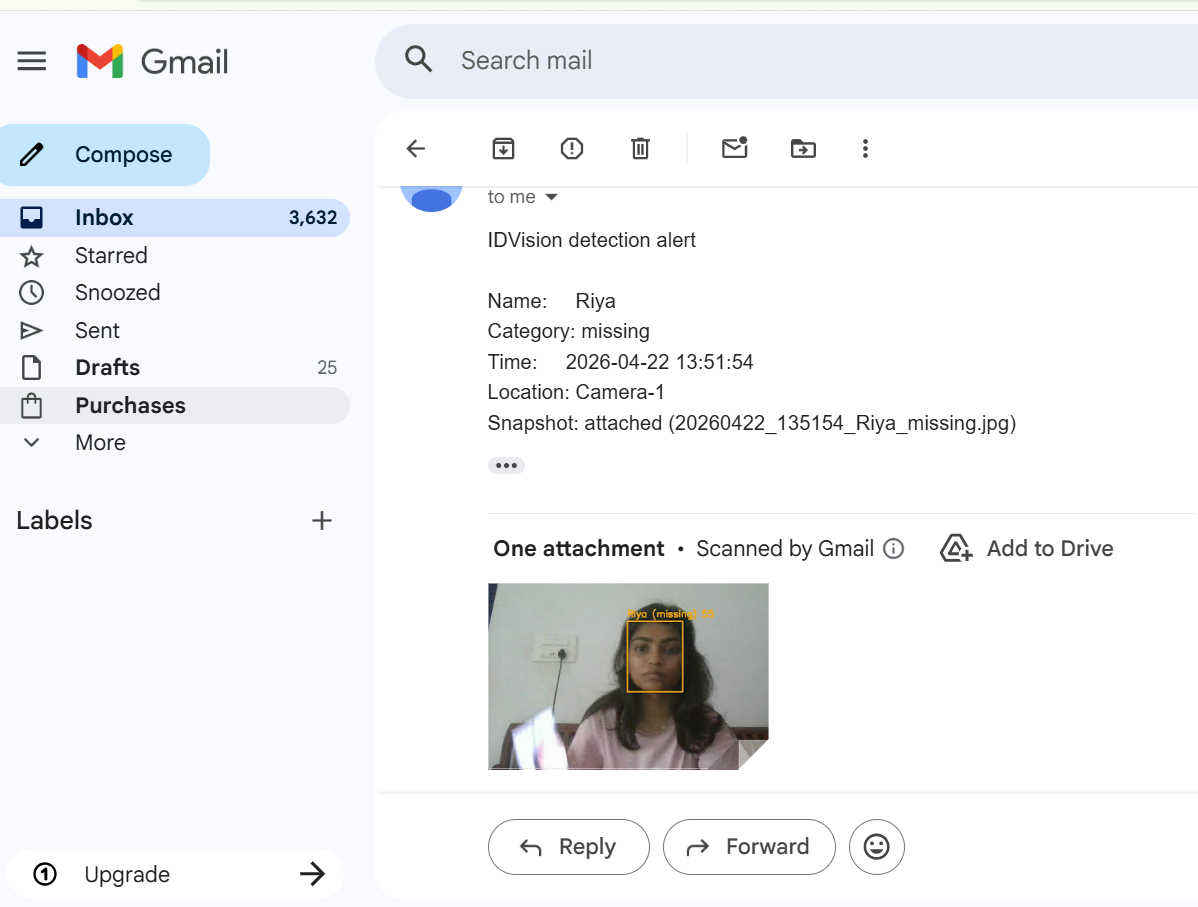
\includegraphics[width=0.85\linewidth]{alert_email.png}
    \caption{A delivered detection email with category, location, timestamp, and the attached snapshot JPEG.}
    \label{fig:ui-email}
\end{figure}

\clearpage
\end{document}
